\documentclass[a4paper,10pt]{book}
\usepackage[utf8]{inputenc}
\usepackage[T2A]{fontenc}
\usepackage[warn]{mathtext}
\usepackage[russian]{babel}
\usepackage{amsmath, amsfonts, amssymb}
\usepackage{caption}
\ifx\pdfoutput\undefined
\usepackage{graphicx}
\else
\usepackage[pdftex]{graphicx}
\fi
\let\vec\mathbf
\setcounter{chapter}{12}
\usepackage{chngcntr}
\counterwithout{figure}{chapter}
\usepackage{fancyhdr}
\pagestyle{fancy}
\renewcommand{\headrulewidth}{0pt}
\fancyhead{}
\fancyhead[LE,RO]{\chaptername\ \thechapter}
\fancyfoot{}
\fancyfoot[LE,RO]{\thepage}


\addto\captionsrussian{\renewcommand{\chaptername}{Лекция}}

\begin{document}
% Раздел 2
% Лекция 13
\part{Раздел II}
\chapter{Понятие о токе}
В предыдущем разделе рассматривались неподвижные электрические заряды и создаваемое ими электрическое поле. Перейдём к изучению движущихся зарядов. Электрическим током называют направленное перемещение заряженных частиц или движение заряженных тел. Ток, образуемый движением заряженных микрочастиц в твердых, жидких или газообразных телах под действием электрического поля называют \emph{током проводимости}. Заряженные частицы, движение которых образует электрический ток, получили название \emph{носителей тока}.

В металлах ток создается движние свободных электронов. В жидкостях носителями тока служат положительные и отрицательные ионы (ионный ток). В газах ток создается движением положительных и отрицательных ионов, а также электронов. Носителями тока в полупроводниках являются электроны и ``дырки'' (свободные места, на которые могут переходить электроны), частично подобные положительные положительным зарядам.

Кроме тока проводимости различают еще \emph{ток в вакуума}, например поток электронов в электронной лампе, телевизионной 
трубке. 

Движение заряженных тел (макроскопических) называют \emph{конвекционным (переносным) током}.

При движении любой заряженной частицы или тела в окружающем пространстве образуется магнитное поле. Поэтому основным свойством 
всякого тока - проводимости, в вакууме и конвекционного - является образование магнитного поля (магнитное действие тока). Прохождение тока в твердых\footnote{За исключением сверхпроводников}, жидких и газообразных телах сопровождается их нагреванием в результате частичного превращения упорядоченного действия тока в хаотическое (тепловое действие тока).

Во всех случаях ионного тока наблюдается перенос вещества и некоторые химические процессы (химическое действие тока).

\section{Сила тока}
Силой тока \emph{(i, I)} называют скалярную величину равную отношению количества электричества \emph{dq}, проходящего через некоторую
поверхность, ко времени прохождения \emph{dt}. Обычно этой поверхностью служит поперечное сечение проводника.
\begin{equation}\label{iless}
 i = \frac{\mathrm{d}q}{\mathrm{d}t}
\end{equation}
Формула \ref{iless} пригодна и для меняющегося и для постоянного тока. Если же сила тока неизменна во времени, то величина её \emph{I} определится как отношение \emph{q} к \emph{t}.
\begin{equation}\label{igreat}
 I = \frac{q}{t}
\end{equation}
Иногда вместо термина ``сила тока'' говорят просто ``ток''.

Единицей силы тока служит ампер (\emph{a}). Определение этой основной единицы Международной системы приведено в разделе ``Электромагнетизм''
(лекция 34).

Из формулы \ref{igreat} можно определить производную единицу заряда в СИ
\begin{equation}
 1 \text{к} = 1 \text{а} \cdot 1 \text{сек} \nonumber
\end{equation}
Один кулон - это заряд, который проходит через сечение проводинка за 1 \emph{сек} при силе тока в 1 \emph{а}. При этом через сечение проводника пройдёт 
\begin{equation}
 N = \frac{1}{e} = \frac{1 \text{к}}{1,6 \cdot 10^-19 \text{к}} = 6,25 \cdot 10^18 \nonumber
\end{equation}
элементарных зарядов.

Формула \ref{igreat} используется в системе СГС для определения единицы силы тока
\begin{equation}\label{sgsamp}
  1\text{СГС}_I = \frac{1\text{СГС}_q}{1 \text{cек}} = \frac{1}{3 \cdot 10^9} \text{а}
\end{equation}
\section{Плотность тока}
В учении о токе важную роль играет векторная величина плотность тока \textbf{j}, численно равная силе тока, отнесенное к единице площади поперечного сечения проводника с током.
\begin{equation}\label{ji}
 j = \frac{I}{S}
\end{equation}
Плотность тока измеряется в $\text{а/м}^2$ (внесистемная единица $1\frac{\text{а}}{\text{мм}^2} = 10^6\frac{\text{а}}{\text{м}^2}$).

Если рассмотреть проводник с переменным сечением или проводящую среду, то плотность тока \emph{j} будет величиной переменной
\begin{equation}\label{dencity}
 j = \frac{\mathbf{d}I}{\mathbf{d}S_n}
\end{equation}
где $dS_n$ - перпендикулярный к направлению плотности тока элемент площади.

Тогда
\begin{equation}\label{inti}
 I = \int\limits_{s}j\mathbf{d}S_n
\end{equation}
т.е. сила тока является потоком от вектора плотности тока через заданную поверхность (см. лекцию 2).
\section{Закон Ома}
В 1827 г. немецкий учитель физики Ом установил опытным путём пропорциональность между напряжением \emph{U}, приложенным к участку цепи, и током, созданным в нём. Отношение напряжения (разности потенциалов) к силе тока в данном участке цепи есть величина
постоянная называемая сопротивлением участка
\begin{equation}\label{resist}
 \frac{U}{I} = R
\end{equation}
Как известно, сопротивление проводника \emph{R} постоянного сечения связанно с его длиной \emph{L}, площадью поперечного сечения \emph{S} и удельным сопротивлением $\rho$ следующим соотношением:
\begin{equation}\label{rls}
 R = \rho\frac{L}{S} = \frac{1}{\gamma}\frac{L}{S}
\end{equation}
Величина, обратная сопротивлению, - $G = \frac{1}{R}$ называется проводимостью, а $\gamma = \frac{1}{\rho}$ - удельной проводимостью
(электропроводимостью).

Из формулы \ref{resist} устанавливается единица для измерения сопротивления в СИ
\begin{equation}
 1 \text{ом} = \frac{1\text{в}}{1\text{a}},
\end{equation}
т.е. 1 \emph{ом} является сопротивлением проводника, в котором идет ток в 1 \emph{а} при напряжении 1\emph{в} между его концами.

Удельное сопротивление $\rho$ численно равно сопротивлению проводника из данного материала, длиной в 1 \emph{м} и поперечным сечением
в 1 $\text{м}^2$ (в СИ); измеряется величина $\rho$ в $\frac{\text{ом} \cdot \text{м}^2}{\text{м}} = \text{ом} \cdot \text{м}$.
Внесистемная единица $1 \text{ом} \cdot \text{см} = 10^-2 \text{ом} \cdot \text{м}$.

Как известно из электростатики, напряженность однородного поля численно равна падению потенциала на единицу расстояния
\begin{equation}\label{Ell}
 E = \frac{U}{L}
\end{equation}
Используя формулы \ref{igreat} \ref{dencity} \ref{resist} \ref{rls} и \ref{Ell}, получаем следующее выражение для плотности тока:
\begin{equation}\label{longf}
 j = \frac{I}{S} = \frac{U}{RS} = \frac{U}{\rho\frac{L}{S}S} = \frac{1}{\rho}\frac{U}{L} = \gamma E
\end{equation}
где \emph{E} - напряженность электрического поля, созданного в проводнике.

Так как \textbf{E} - величина векторная, то
\begin{equation}\label{vecj}
 \vec{j} = \gamma\vec{E}
\end{equation}
т.е. вектор \textbf{j} совпадает по направлению с вектором напряженности электрического поля.

Формула \ref{vecj} выражает закон Ома в \emph{дифференциальной форме}. Величина силы тока получается в общем случае путем интегрирования
плотности тока по площади [см. формулу \ref{inti}]. Плотность тока оказывается прямопропорциональной напряженности поля, созданного в проводнике.
\section{Работа и мощность тока. Закон Джоуля-Ленца в дифференциальной форме}
При прохождении тока по проводнику совершается работа по перенесению заряда q между точками с разностью потенциалов \emph{U}. Эта работа 
затрачивается на нагревание проводника
\begin{equation}\label{work}
 A = qU = IUt = I^2Rt = \frac{U^2}{R}t = Q
\end{equation}
В Международной системе единиц работа \emph{A} и количество тепла \emph{Q} измеряются в джоулях. Поэтому формула \ref{work} для работы 
тока одновременно выражает закон Джоуля-Ленца о тепловом действии тока. 

Заметим, что при \emph{последовательном} соединении сила тока \emph{I} во всех сечениях одинакова и поэтому, согласно формуле $Q = I^2Rt$,
количество тепла , выделяющееся на каком-либо участке цепи, пропорционально его сопротивлению $R$.

При \emph{параллельном} соединении во всех ветвях имеется общее напряжение U и количество тепла
\begin{equation}
 Q = \frac{U^2}{R}t, \nonumber
\end{equation}
выделяющееся в какой-либо ветви, обратно пропорционально ее сопротивлению, т.е. пропорционально ее проводимости.

Подсчитаем количество тепла, выделяемое за единицу времени в единице объема $V$ проводника, т.е. найдём 
\begin{equation}
 Q_1 = \frac{Q}{tV} = \frac{Q}{tSL}. \nonumber
\end{equation}
Используя соотношения \ref{rls}, \ref{Ell} и \ref{work}, получаем:
\begin{equation}\label{warm}
 Q_1 = \frac{U^2}{RSL} = \frac{E^2L^2}{\frac{1}{\gamma}\frac{L}{S}SL} = \gamma E^2.
\end{equation}
\emph{Колличество тепла, выделяемое в единице объема проводника за единицу времени, пропорционально квадрату напряженности электрического поля созданного в проводнике.}

Соотношение \ref{warm} называется законом Джоуля-Ленца в дифференциальной форме, так как определяет количество тепла, выделяемое в 1 сек в единице объема.

В общем случае количнство тепла, выделяемое в 1 сек во всем объеме,
\begin{equation}\label{warmVol}
 Q_V = \int\limits_{(V)}Q_1\mathbf{d}V
\end{equation}
Рассматривая формулы \ref{vecj} и \ref{warm}, замечаем, какую важную роль играет величина напряженности электрического поля $E$, созданного источником в проводнике. Величина $E$ определяет плотность тока в цепи и количество выделяемого током тепла.
\chapter{Замкнутая цепь с источником тока}
Рассмотрим замкнутую цепь электрического тока, составленную из источника тока и внешнего сопротивления $R$ \ref{img1}. Во внешней части цепи заряды движутся под действием электростатических сил от большего потенциала к меньшему (путь $1R2$). Для того чтобы заставить заряды двигаться внутри источника тока против направления электростатического поля (от 2 к 1 через внутренней сопротивление $r$), необходимо наличие сил неэлектрического происхождения, так называемых сторонних сил.

Величину, определяемую работой, которую совершают сторонние силы при перемещении единичного положительного заряда по всей замкнутой цепи, называют электродвижущей силой (э. д. с.) $\mathcal{E}$ в этой цепи (не путать с напряженностью электрического поля $\mathbf{E}$ и ее числовым значением $E$).
\begin{equation}\label{eds}
 \mathcal{E} = \frac{A_\text{ст}}{q_0}
\end{equation}
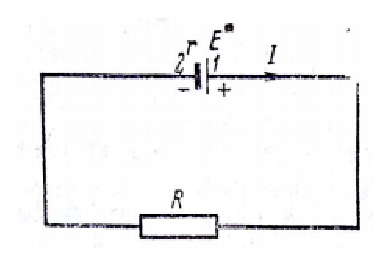
\includegraphics{img1}
Этой работой измеряется электростатическая энергия, которая получается в источнике тока за счет иных, неэлектрических форм энергии.

Из определения ЭДС видно, что это величина, аналогичная разности потенциалов (напряжению), имещая ту же размерность и измеряемая в тех же
единицах -- вольтах.

Падение напряжения во внешней части цепи $U_1$ измеряется работой, совершаемой при перемещении единичного положительного заряда через внешнее сопротивление $R$
\begin{equation}\label{u1}
 U_1 = \frac{A_1}{q_0}
\end{equation}
При прохождении тока по всей замкнутой цепи внутри источника также затрачивается энергия на продвижение зарядов и имеет место внутреннее падение напряжения $U_2$ эта энергия превращается в джоулево тепло внутри источника.
\begin{equation}\label{u2}
 U_2 = \frac{A_2}{q_0}
\end{equation}
Учитывая, что все три величины - $\mathcal{E}, U_1, \text{и} U_2$ измеряются работой по перемещению единичного положительного заряда и применяя закон сохранения энергии, получим
\begin{equation}\label{Aex}
 A_\text{ст} = A_1 + A_2
\end{equation}
\begin{equation}\label{Aex/q0}
 \frac{A_\text{ст}}{q_0} = \frac{A_1}{q_0} + \frac{A_2}{q_0} \text{ и } \mathcal{E} = U_1 + U_2.
\end{equation}
Эдс равна сумме падений напряжения во внешней и внутренней частях замкнутой цепи.

Устройства, в которых сторонние силы совершают работы и происходит превращение какого-либо вида энергии в электрическую, называются генераторами, или источниками эдс (реже - источниками тока).

Подавляющая часть электрической энергии совершается за счет совершения механической работы в машинах, где используется явление электромагнитной индукции (генераторы на стационарных и передвижных электростанциях). В термоэлементах (термопарах) происходит превращение тепловой энергии в электрическую. В гальванических элементах и аккумуляторах химическая энергия преобразуется в электрическую. Некоторые виды фотоэлементов позволяют получать эдс за счет лучистой энергии.

Таким образом, следует различать электромеханические, тепловые, химические и оптические генераторы, или источники эдс. В настоящее время разрабатываются новые генераторы -- магнитогидродинаические, где тепловая энергия нагретого ионизированного газа или дыма непосредственно превращается в электрическую.

Получение различных радиоактивных изотопов позволило создать маломощные генераторы длительного действия; в них эдс получается за счет непрерывного выбрасывания электронов радиоактивными ядрами.
\section{Закон Ома для всей цепи}
Используя закон Ома для участка цепи, можно заменить в формуле \ref{Aex/q0} $U_1$ и $U_2$ следующими выражениями:
\begin{equation}
 U_1 = IR,\text{ }U_2 = Ir.\nonumber
\end{equation}
Тогда соотношение \ref{Aex/q0} превратится в закон Ома для всей цепи: 
\begin{equation}\label{full_Ohm}
 \frac{\mathcal{E}}{I} = R + r
\end{equation}
Отношение эдс, действующей в замкнутой цепи, к силе тока есть величина постоянная, равная полному сопротивлению цепи или 
\begin{equation}\label{full_I}
 I = \frac{\mathcal{E}}{R + r}.
\end{equation}
Максимальный ток $I_\text{к.з.}$, как следует из закона Ома, получится если внешнее сопротивление R = 0, т.е. имеет место короткое замыкание
\begin{equation}\label{I_shcut}
 I_\text{к.з.} = \frac{\mathcal{E}}{r}
\end{equation}
Записав формулу \ref{full_Ohm} в виде
\begin{equation}
 \mathcal{E} = U_1 + Ir\nonumber
\end{equation}
можно определить эдс как величину, численно равную напряжению на зажимах источника при $I = 0$, т.е. при разомкнутой внешней цепи. Этим пользуются для практического измерения эдс. Точное измерение эдс производится компенсационным способом (известным из лабораторной работы), при котором ток от источника не потребляется. Приближенно эдс измеряется вольтметром с большим сопротивлением.
\section{Полная и полезная мощноть. КПД источника}
Мощность, выделяемая во внешней цепи (нагрузке $R$), называется полезной
\begin{equation}
 P_1 = U_1I = I^2R\nonumber
\end{equation}
Внутри источника тока расходуется мощность 
\begin{equation}
 P_2 = I^2r\nonumber
\end{equation}
Полная мощность замкнутой цепи
\begin{equation}\label{full_P}
 P_n = I^2R + I^2r = IU_1 + IU_2 = I\mathcal{E}.
\end{equation}
Найдем условие, при котором полезная мощность будет максимальной. Для этого выразим полезную мощность как 
\begin{equation}
 P_1 = P_n - P_2 = I\mathcal{E} - I^2r\nonumber
\end{equation}
и приравняем нулю производную
\begin{equation}
 \frac{\mathbf{d}P_1}{\mathbf{d}I} = \mathcal{E} - 2Ir = 0,\nonumber
\end{equation}
откуда
\begin{equation}\label{profit_I}
 I = \frac{\mathcal{E}}{2r}.
\end{equation}
Сравнивая эту формулу с законом Ома \ref{full_I}, видим, что максимальна мощность во внешней цепи выделяется при равенстве внешнего и 
внутреннего сопротивления:
\begin{equation}\label{exeqin}
 R = r.
\end{equation}
Коэффициентом полезного действия $\eta$ источника эдс называется отношение полезной мощности к полной
\begin{equation}\label{nu}
 \eta = \frac{P_1}{P_n} = \frac{I^2R}{I^2(R + r)} = \frac{U_1}{\mathcal{E}} = \frac{R}{R + r}
\end{equation}
Наибольший кпд, равный единице, получится при равенстве нулю внутреннего сопротивления источника. Исходя из этого стараются делать внутреннее сопротивление источника эдс (обмоток механического генератора, электролита и пластин аккумулятора) минимальным.
\section{Правила Кирхгофа}
Для расчета сложных электрических цепей удобно применять правила, установленные немецким физиком Кирхгофом. Первое из них относится к точке разветвления - узлу \ref{img2} : \emph{алгебраическая сумма сил токов, сходящихся в узле, равна нулю}.
\begin{equation}\label{kirchgoff1}
 \sum_1^n I_k = 0
\end{equation}
Приходящие к узлу токи считаются положительными, а уходящие -- отрицательными. Применив первое правило Кирхгофа к узлу, изображенному на рис. 25, получим следующее выражение:
\begin{equation}
 I_1 - I_2 + I_3 - I_4 - I_5 = 0\nonumber
\end{equation}
По существу первое правило Кирхгофа выражает тот факт, что при установившемся токе заряды не могут скапливаться в узлах.

Второе правило Кирхгофа является обобщением закона Ома для всей цепи на случай наличия нескольких связанных контуров. Согласно этому правилу \emph{при обходе замкнутого контура алгебраическая сумма произведений токов на соответствующие сопротивления (сумма падения напряжений) равна алгебраической сумме э.д.с.}, т.е. при полном обходе замкнутого контура сумма подъемов и падений потенциала равна нулю.
\begin{equation}\label{kirchgoff2}
 \sum_1^n I_kR_k = \sum_1^m\mathcal{E}_i.
\end{equation}
При использовании правил Кирхгофа необходимо иметь в виду следующее:
\begin{enumerate}
 \item предварительно на схеме указывается предположительное направление токов;
 \item направление обхода контуров выбирается произвольно и сохраняется неизменным при решении задач;
 \item если направление данного тока совпадает с направлением обхода контура, то падение напряжения $IR$ считается положительным;
 \item э.д.с. считается положительной, если обход внутри данного источника совершается от отрицательного полюса к положительному;
 \item если после решения уравнений у какого-либо тока получается знак минус, то это означает, что его истинное направление противоположно выбранному;
 \item общее число независимых уравнений, составленных на основании обоих правил Кирхгофа, должно равняться числу токов в данной схеме
\end{enumerate}

Применим правила Кирхгофа к схеме, изображенной на \ref{img3}.

\textbf{Первое правило.} Его следует применять в узле $A$, или в узле $B$. Для узла $B$ имеем:
\begin{equation}\label{kirex1}
 I_1 + I_2 - I_3 = 0.
\end{equation}
Уравнение для узла $A$ идентично.

\textbf{Второе правило.} Выберем направление обхода, например, по часовой стрелке:
\begin{equation}\label{kirex2}
 \begin{cases}
    I_1R_1 + I_1r_1 - I_2r_2 - I_2R_2 = \mathcal{E}_1 - \mathcal{E}_2 \;\;\;\;\;\;\;(\text{Контур} A\mathcal{E}_1B\mathcal{E}_2A)\\
    I_2R_2 + I_2r_2 + I_3R_3 + I_3r_3 = \mathcal{E}_2 + \mathcal{E}_3 \;\;\;\;\;\;\;(\text{Контур} A\mathcal{E}_2B\mathcal{E}_3A)
 \end{cases}
\end{equation}
%img3 
Решая совместно \ref{kirex1} и \ref{kirex2}, найдем токи $I_1$, $I_2$ и $I_3$ (сопротивления и э.д.с. обычно известны).

Если бы мы составили третье уравнение  второму правилу Кирхгофа, а именно, обошли контур $A\mathcal{E}_1BR_3A$, то полученное уравнение явилось бы следствием первых двух.
\chapter{Основные положения корпускулярной теории проводимости}
Как было сказано, током проводимости называют ток, созданный направленным движением электрически заряженных частиц - корпускул - в твердых телах, жидкостях или газах.
 
Рассмотрим проводник длиной $L$ с площадью поперечного сечения $S$ (\ref{img4}). Концентрацию носителей тока, т.е. число заряженных частиц в единице объема обозначим $n$, а заряд каждого носителя $q_0$. Если приложить к проводнику напряжение $U$, то под действием созданного в проводнике электрического поля на быстрое, хаотическое тепловое движение носителей наложится медленное, направленное перемещение их вдоль поля со средней скоростью $v$. Если за время $t$ облак заряженных частиц переместилось на расстояние $L$, то очевидно $v = \frac{L}{t}$. За время $t$ через сечение проводника пройдут все заряды, находящиеся в части объема проводника $S\cdot L = V$. Поэтому учитывая, что концентрация
%img4
носителей n, а заряд каждого из них $q_0$, общая величина заряда $q$, перенесенного через сечение проводника за время $t$, выразим произведением
\begin{equation}\label{full_q}
 q = q_0nSL.
\end{equation}
Отсюда плотность тока
\begin{equation}\label{density}
 j = \frac{I}{S} = \frac{q}{tS} = \frac{q_0nSL}{tS} = q_0nv
\end{equation}
[см. формулы \ref{igreat}, \ref{ji}, \ref{full_q}].

Таким образом, \emph{плотность тока проводимости пропорциональна заряду каждого носителя, концентрации и средней скорости направленного движения носителей тока.} Как было сказано, плотность тока - векторная величина и по направлению совпадает с вектором скорости $\mathbf{v}$.

При наличии различных заряженных частиц - электронов, ионов, <<дырок>> - общая плотность тока
\begin{equation}\label{job}
 j = \sum_1^mj_i,
\end{equation}
где $j_i$ - плотность тока, создаваемого каждым из $m$ носителей.

В простейшем случае двух носиетелей, например положительных и отрицательных ионов, или <<дырок>> и электронов
\begin{equation*}
 j = j_+ + j_-
\end{equation*}
или
\begin{equation}\label{j154}
  j = q_{0+}n_+v_+ + q_{0-}n_-v_-
\end{equation}
В формуле (\ref{j154}) $q_{0+}$ и $q_{0-}$ - заряды положительных и отрицательных носителей, $n_+$ и $n_-$ - концетрация их, $v_+$ и $v_-$ 
- средние скорости.
\section{Подвижность носителей}
На заряженную частицу, участвующую в образовании тока проводимости, действует со стороны электрического поля, напряженность которого $E$, сила
\begin{equation}\label{155}
 F_\text{эл} = q_0E,
\end{equation}
ускоряющая эту частицу. При движении каждый носитель тока взаимодействует путем столкновения с другими частицами среды, передавая им некоторый импульс. В результате такого процесса среда тормозит движение носителя. Действующая при этом сила трения (сопротивления)
\begin{equation}\label{156}
 F_\text{тр} = kv
\end{equation}
предположительно может считаться пропорциональной средней скорости частицы. Например, при движении ионов в жидкости картина уподобляется движению шарика в вязкой среде, и сила трения определяется известной из молекулярной физики формулой Стокса
\begin{equation}
 F_\text{тр} = 6\pi \eta r v, 
\end{equation}
где $\eta$ - коэффициент вязкости среды, а r - радиус движущегося шарика.
Сравнивая формулу Стокса с выражением (\ref{156}), видим, что $k = 6\pi \eta r$, т.е. коэффициент трения $k$ зависит от вязкости (а следовательно, 
от температуры) и от размеров частицы.

При установившемся движении 
\begin{equation*}
 F_\text{эл} = F_\text{тр}.
\end{equation*}
Используя (\ref{155}) и (\ref{156}), получим 
\begin{equation}\label{157}
 q_0E = kv
\end{equation}
Величина $u$, численно равная средней скорости, с которой заряженная частица движется в данной среде под действием электрического поля с 
напряженностью, равной единице, называется подвижностью тока в данной среде 
\begin{equation}\label{158}
 u = \frac{v}{E} = \frac{q_0}{k}
\end{equation}
Используя определение подвижности (\ref{158}) и формулу (\ref{j154}), получим следующую формулу для плотности тока при наличии двух носителей
противоположных знаков:
\begin{equation}\label{159}
 j = q_{0+}n_+v_+ + q_{0-}n_-v_- = (q_{0+}n_+u_+ + q_{0-}n_-u_-)E.
\end{equation}
Сравнивая формулу (\ref{159}) для плотности тока с законом Ома в дифференциальной форме $j = \gamma E$, видим, что роль электропроводности играет
коэффициент при величине $E$
\begin{equation}\label{1510}
 \gamma = (q_{0+}n_+u_+ + q_{0-}n_-u_-).
\end{equation}
В СИ единицей подвижности является $1\frac{\text{м}}{\text{сек}}:1\frac{\text{в}}{\text{м}} = 1\frac{\text{м}^2}{\text{в}\cdot\text{сек}}$.
\section{Опытные предпосылки классической электронной теории металов}
В 1901 г. Рике доказал на опытах, что прохождение тока через металл не связано с переносом атомов металла. Через три цилиндрических проводника
, изготовленных из различных металлов и плотно прижатых друг к другу хорошо отшлифованными основаниями, пропускался постоянный ток. Опыт продолжался
свыше года, после чего цилиндры разобрали и проанализировали. Вес их не изменился, а химический состав в прилегавших областях изменился не больше, чем 
при обычной диффузии атомов в твердых телах. Этот опыт показывает, что атомы (ионы) металла не участвуют в создании тока.

Доказательством того, что носителями тока в металле являются именно электроны, служат опыты по обнаружению инерциального движения электронов.
Стюарт и Толмен (1916 г.) вращали проволочную катушку, имевшую длину провода $L$, с большой линейной скоростью $v$; свободные электроны вращались
вместе с катушкой. Затем катушку резко тормозили; электроны по инерции продолжали двигаться в прежнем направлении, причем их упорядоченное движение
делалось хаотическим, а кинетическая энергия превращалась в джоулево тепло
\begin{equation}\label{1511}
 -\mathbf{d}W_\text{к} = \mathbf{d}Q.
\end{equation}
Изменение кинетической энергии одного электрона
\begin{equation}\label{1512}
 \mathbf{d}(\frac{mv^2}{2}) = mv\mathbf{d}v,
\end{equation}
а их число в проволоке катушки $n\cdot S\cdot L$. Поэтому 
\begin{equation}\label{1513}
 dW_\text{к} = nSLmv\mathbf{d}v.
\end{equation}
Вспомнив, что $I = j \cdot S = envS$, заменим в выражении (\ref{1513}) произведение $nvS$ значением $\frac{I}{e}$, где $e$ - заряд электрона.

Используя равенства (\ref{1511}), (\ref{1513}) и закон Джоуля-Ленца, получаем:
\begin{equation}\label{1514}
 \mathbf{d}W_\text{k} = -I\frac{m}{e}L\mathbf{d}v = \mathbf{d}Q = I^2R\mathbf{d}t.
\end{equation}
Сокращаем на $I$ и заменяем на $I\cdot \mathbf{d}t = \mathbf{d}q$
\begin{equation}\label{1515}
 -\frac{m}{e}L\mathbf{d}v = R\mathbf{d}q.
\end{equation}
Интегрируем выражение (\ref{1515}), учитывая что скорость электронов изменяется от $v$ до $0$ (при торможении) и при этом по цепи протекает заряд
$q$:
\begin{equation*}
 -\frac{m}{e}L\int_v^0\mathbf{d}v = R\int_0^q\mathbf{d}q.
\end{equation*}
Отсюда
\begin{equation}\label{1516}
 \frac{m}{e}Lv = Rq \;\text{и}\;\frac{e}{m}=\frac{Lv}{Rq}.
\end{equation}
Длина проволоки катушки L и начальная скорость её вращения $v$ известны. Замыкая катушку на баллистический гальванометр (об этом приборе см. лекцию 40),
по его отбросу измеряют заряд $q$, протекший по цепи. Сопротивление катушки и гальванометра также известно. Таким образом, из опытных данных
может быть найдено отношение $\frac{e}{m}$, которое достаточно точно совпадает с числом, определенным из других опытов для свободных электронов.

В начале XX века физики Лоренц и Друде разработали классическую электронную теорию металлов. Атомы, образующие кристаллическую решетку металла, 
находятся на близких расстояниях и между ними действуют значительные электрические силы. Вследствие этого, валентные электроны отрываются от своих
атомов, оставляя в узлах решетки положительные ионы. Эти <<свободные>> электроны двигаются хаотически, взаимодействуя друг с другом и с ионами
решетки. Хотя силы этого взаимодействия велики, но средняя сила, действующая на данный свободный электрон со стороны остальных электронов и 
ионов, близка к нулю. Поэтому электроны, оторванные от атомов, считаются свободными. Их взаимодействие с ионами и другими электронами сводится к столкновениям.
При этом частицы обмениваются импульсом, энергией.

Лоренц и Друде предположили, что свободные электроны в металле представляют собой <<электронный газ>>, подчиняющийся законам, установленным
для молекул идеального газа; скорости свободных электронов распределяются согласно статистическому закону Максвелла-Больцмана (см. раздел 
<<Молекулярная физика>>).

По этой теории средняя кинетическая энергия свободных электронов определяется формулой энергии молекул газа
\begin{equation}\label{1517}
 \frac{mu^2_T}{2} = \frac{3}{2}kT.
\end{equation}
Впоследствии оказалось, что теория Друде и Лоренца не лишена принципиальных недостатков, так как энергия и скорости электронов подчиняются 
другому, более сложному закону (см. лекцию 17). Тем не менее классическая электронная теория сыграла известную положительную роль, позволив 
объяснить такие важные опытные законы, как закон Ома и Джоуля-Ленца.
\chapter{Электронная теория проводимости металлов}
Рассматривая согласно классической электронной теории металлов свободные электроны как электронный газ, можно вывести законы Ома и Джоуля-Ленца.

Рассмотрим объем проводника длиной $L$ и сечением $S$ (рис. \ref{img5}). Свободные электроны участвуют в тепловом движении, имея средние квадратичные
скорости
\begin{equation}\label{161}
 u_T = \sqrt{\frac{3kT}{m}},
\end{equation}
определяемые по формуле для скорости молекул газа. Подстановкой в формулу (\ref{161}) массы электрона $m = 9,1\cdot 10^{-31}\text{кг}$ и 
постоянной Больцмана $k = 1,38 \cdot 10^{-23} \emph{дж/град}$, получим для комнатной температуры $t = 17^\circ C$ 
или $T = 290^\circ K$ величину средней тепловой скорости электронов в металле порядка $100 \emph{км/сек}$.

Если на электроны подействует электрическое поле, то на их хаотическое тепловое движение наложится упорядоченное движение со средней скоростью
$v$, значительно меньшей тепловой скорости.

Действительно, при плотности тока в проводнике, равной, например, $5\emph{а/мм}^2 = 5\cdot 10^6 a/\text{м}^2$ и при концентрации свободных
электронов 
\begin{equation*}
 n \approx 10^{23} \cdot 1/\text{см}^3 = 10^{29} \cdot 1/\text{м}^3,
\end{equation*}
получим из известной формулы
\begin{equation*}
 j = nq_0v,
\end{equation*}
где $q_0$ равно заряду электрона $e = 1,6 \cdot 10^{-19}\text{к}$, 
\begin{equation*}
 v = \frac{j}{ne} = \frac{5 \cdot 10^6}{10^29\cdot 1,6 \cdot 10^{-19}} = 3 \cdot 10^{-4} \frac{\text{м}}{\text{сек}} = 0,3 \frac{\text{мм}}{\text{сек}}.
\end{equation*}
Это упорядоченное движение электронов и образует ток в металле.
\section{Вывод закона Ома из электронной теории}
Рассмотрим движение свободного электрона в металле. После упругого удара об ион 1 (\ref{img6}) электрон отскочит от него, имея тепловую скорость
$u_T$, и полетит к иону 2.

За время свободного полета $\tau$ между двумя столкновениями с ионами на электрон, имеющий заряд $e$, со стороны электрического поля будет
действовать постоянная сила $F$.
%img 6
\begin{equation}\label{162}
 F = eE
\end{equation}
Под действием этой силы электрон будет двигаться равноускоренно и к моменту столкновения с ионом 2 скорость направленного движения электрона
станет равной $v_\tau$. Заметим, что после столкновения электронов с ионами средняя начальная скорость является тепловой ($u_T$). Это значит, 
что в результате столкновения электрон передал иону дополнительную кинетическую энергию, полученную в поле. Поэтому средняя начальная скорость
упорядоченного движения электрона $v_0 = 0$.

Среднее расстояние между ионами, с которыми электрон испытывает столкновения, является средней длиной свободного пробега.
\begin{equation}\label{163}
 \lambda = u_T\tau
\end{equation}
Хотя скорость электрона изменяется во время свободного пробега, как было показано, $v \ll u_T$ и при определении времени движения электрона
между двумя столкновениями считаем его скорость постоянной и равной $u_T$.

Ускорение $a$, которое приобретает электрон под действием силы поля,
\begin{equation*}
 a = \frac{F}{m} = \frac{eE}{m},
\end{equation*}
а скорость 
\begin{equation}\label{164}
 v_T = a_T = \frac{eE}{m}\tau = \frac{eE}{m} \cdot \frac{\lambda}{u_T}.
\end{equation}
Средняя скорость упорядоченного движения электрона
\begin{equation}\label{165}
 v = \frac{v_0 + v_\tau}{2} = \frac{eE\lambda}{2mu_T}
\end{equation}
Подставим выражение, полученное для средней скорости направленного движения электрона, в выведенную ранее формулу плотности тока (\ref{density}).
Заряд носителя тока $q_0$ в данном случае является зарядом электрона $e$
\begin{equation}\label{166}
 j = ne\frac{eE\lambda}{2mu_T} = \frac{ne^2\lambda}{2mu_T}E.
\end{equation}
Сравнивая выведенную формулу с законом Ома в дифференциальной форме, видим, что соотношение (\ref{166}) превратится в этот закон, если положить
\begin{equation}\label{167}
 \gamma = \frac{1}{\rho} = \frac{ne^2\lambda}{2mu_T}.
\end{equation}
Выражение (\ref{167}) дает зависимость сопротивления металлов от температуры. Формула
\begin{equation}\label{167a}
 \rho = \frac{2mu_T}{ne^2\lambda}
\end{equation}
для удельного сопротивления позволяет качественно оценить температурную зависимость: при повышении температуры скорость теплового движения
возрастает [см. (\ref{161})], а длина свободного пробега электронов уменьшается вследствие того, что при нагреве амплитуда колебаний ионов
кристаллической решетки металлов увеличивается и возрастает число столкновений электронов с ионами; таким образом $\lambda$ убывает. Увеличение
$\lambda$ вследствие расширения металла пренебрежимо мало. Точная зависимость $\lambda$ от температуры неизвестно и это не позволяет получить
соотношение ежду удельным сопротивлением $\rho$ и температурой. 

Анализ формулы (\ref{167a}) показывает, что сопротивление металлов должно расти с увеличением температуры; это и имеет место в действителньости.

Экспериментально установлено, что удельное сопротивление металла $\rho$ линейно зависит от температуры
\begin{equation}\label{168}
 \rho_t = \rho_0(1 + \alpha t^\circ),
\end{equation}
где $\rho_0$ - удельное сопротивление при $0^\circ C$, а $\alpha$ - температурный коэффициент сопротивления, различных для разных металлов;
в грубом приближении он близок к $1/273\cdot1/\text{град}$.Поэтому
\begin{equation}\label{168a}
 \rho_t = \rho_0(1 + \frac{1}{273}t^\circ) = \rho_0 \frac{273 + t^\circ}{273} = \rho_0\frac{T}{T_0}.
\end{equation}
В заключение заметим, что у электролитов, полупроводников и диэлектриков при повышении температуры сопротивление резко падает, так как увеличивается
число носителей тока. Кроме того, у электролитов резко возрастает подвижность ионов вследствие уменьшения вязкости с температурой.
\section{Сверхпроводимость}
Линейная зависимость удельного сопротивления от температуры изображена на рис \ref{img7} (линия $0a$).
%img7
Однако, проводя опыты с чистыми металлами,
голландский физик Камерлинг-Оннес в 1911 г., обнаружил у некоторых из них резкое, скачкообразное уменьшение сопротивления при температурах,
строго определенных для каждого металла и находящихся в интервалах от $1$ до $10^\circ$ K (см., например точки $T_{c1}$ и $T_{c2}$ для двух
металлов). Это явление было названо сверхпроводимостью. Если в проводнике, находящемся в сверхпроводящем состоянии, будет возбуждён ток,
то он будет протекать (без внешней э.д.с.) в течение сотен часов, заметно не убывая. Если сверхпроводник поместить в сильное магнитное поле 
(в том числе магнитное поле тока значительной силы, идущего по сверхпроводнику), то сверхпроводящее состояние разрушается. Дальейшие исследования
показали, что сверхпроводимость наблюдается не только у чистых металлов (Al, Zn, Cd, Sn, Pb, Nb, U и др.), но и у сплавов и соединений, в 
том числе у сплавов из несверхпроводящих элементов. У нитрида ниобия (NbN) падение сопротивления наблюдается при $T = 23^\circ K$.

В настоящее время ведутся усиленные поиски искусственно создаваемых веществ, у которых сверхпроводимость наблюдалась бы при возможно более
высоких температурах. Открытие таких веществ позволило бы создавать сверхпроводящие элементы электро и радиотехнических устройств, обладающих
весьма ценными практическими свойствами, в том числе ничтожным потреблением энергии.
\section{Вывод закона Джоуля-Ленца из электронных представлений}
Закон Джоуля-Ленца также легко выводится на основе классической электронной теории. Нагрев проводника при прохождении по нему тока объясняется тем, 
что электроны, ускоренные полем, при столкновениях с ионами кристаллической решетки отдают им полученную дополнительную кинетическую энергию.
Для одного электрона эта энергия равна
\begin{equation}\label{169}
 W_1 = \frac{mv_\tau^2}{2}
\end{equation}
Где $v_\tau$ - конечная скорость, полученная за счет разгона электрическим полем. В \emph{1 сек} электрон испытывает в среднем $Z$ столкновений
\begin{equation}\label{1610}
 Z = \frac{U_T}{\lambda}
\end{equation}
(см. раздел <<Моллекулярная физика>>).

Число столкновений за $t$ секунд составляет $Z\cdot t$. Во всем объеме проводника число свободных электронов $nSL$ (где $n$ - концентрация 
свободных электронов). Окончательно дополнительную энергию, переданную за $t$ сек всеми свободными электронами ионам, получим умножением 
$W_1$ на $Zt$ и на $nSL$.
\begin{equation}\label{1611}
 W = \frac{mv^2_\tau}{2}ZtnSL
\end{equation}
Заменяем $v_\tau$ и $Z$ согласно (\ref{164}) и (\ref{1610})
\begin{equation*}
 W = \frac{me^2E^2\lambda^2}{2m^2u_T^2}\cdot\frac{u_T}{\lambda}nSLt = \frac{ne^2\lambda}{2mu_T}SLtE^2.
\end{equation*}
Но 
\begin{equation*}
 \frac{ne^2\lambda}{2mu_T} = \gamma;
\end{equation*}
тогда
\begin{equation}\label{1612}
 W = \gamma E^2SLt.
\end{equation}
Количество тепла $Q_1$, которое выделяется в 1 \emph{сек} в единице объема $V = L\cdot S$ проводника, будет
\begin{equation}\label{1613}
 Q_1 = \frac{W}{SLt} = \frac{Q}{SLt} = \gamma E^2.
\end{equation}
Полученное выражение и представляет собой закон Джоуля-Ленца в дифференциальной форме(см. лекцию 13).
\section{Затруднения классической электронной теории}
Полученная на основе классической электронной теории формула для зависимости удельного сопротивления от температуры (\ref{167a}) не дает 
возможности, как уже указывалось, получить экспериментальное соотношение (\ref{168a}).

Явление сверхпроводимости совершенно не укладывается в рамки теории Друде и Лоренца. Кроме того, в рамках классической теории оказалось 
невозможным объяснить величину теплоемкости металлов, равную согласно опытам $25 \text{кдж}/\text{кмоль}\cdot\text{град}$ (см. закон 
Дюлонга и Пти, лекция 44 по разделу <<Моллекулярная физика>>).

Согласно классическим представлениям общая теплоемкость металла $C_V$ должна складываться из теплоемкости металлической ионной решетки
\begin{equation*}
 C'_V = \frac{6}{2}R = 25\frac{\text{кдж}}{\text{кмоль}\cdot\text{град}}
\end{equation*}
и теплоемкости электронного газа
\begin{equation*}
 C''_V = \frac{3}{2}R = 12,5\frac{\text{кдж}}{\text{кмоль}\cdot\text{град}},
\end{equation*}
рассчитанной как для одноатомного газа. Однако теоретическое значение теплоемкости
\begin{equation*}
 C_V = C'_V + C''_V = 37,5 \frac{\text{кдж}}{\text{кмоль}\cdot\text{град}}
\end{equation*}
резко расходится с приведенным опытным. Оказывается, что электронный газ не влияет на значение теплоемкости, как будто энергия электронов
не зависит от температуры.

Указанные затруднения электронной теории устраняются квантовой теорией электропроводимости твердых тел (см. лекцию 17).
\chapter{О квантовой теории электропроводности}
Обращаясь к выяснению причин расхождения результатов классической электронной теории проводимости металлов с опытными данными, надо прежде всего подчеркнуть, что эти расхождения возрастают при уточнении расчетов и исходных модельных представлений. Это же было установлено в молекулярной физике при изучение теплоемкости газов и твердых тел. Там указывалось, что законы классической механики и статистики лишь весьма ограничено и приблизительно применимы для решения вопросов молекулярной физики. Так, в области обычных температур результаты классической теории теплоемкости приближенно совпадают с опытными данными, а при достаточно низких и высоких температурах резко расходятся с ними.

Развитие физики привело к открытию необычных черт микромира и к созданию количественной теории с соответствующим математическим аппаратом, получившей название квантовой механики. Ниже изложены некоторые представления этой теории и результаты, относящиеся главным образом к электронной проводимости твердых тел.

Квантовая теория твердого тела позволила более глубоко объяснить электрические, тепловые и другие свойства металлов, электронных полупроводников и кристаллических диэлектриков, что способствовало расширению области применения полупроводников в технике.

Согласно квантовой теории частицы, находящиеся под водействием полей, созданных другими частицами или телами, т.е. обладающие не только кинетической, но и потенциальной энергией, могут совершать лишь группу движений, обсуловленных природой частицы и характером поля, в котором она движется, причем переход от одного типа движения к другому может осуществляться лишь скачком (промежуточные, или переходные типы движения отсутствуют).

Иными словами, всякая ограниченная физическая система может пребывать лишь в некоторых определённых состояниях, зависящих от её природы и называемых квантовыми состояниями. Эти состояния, <<дозволенные>> физической природой системы, характеризуются определенными значениями энергии, количества движения (или импульса), момента количества движения и других связанных с ними механических величин. Поэтому одной из основных задач квантовой механики является определение возможных, или <<разрешённых>> значений энергии, или <<энергетических уровней>>, которые выражают полную энергию (а не составляющие её слагаемые - потенциальную или кинетическую). Термин <<энергетические уровни>> возник потому, что <<разрешённые>> значения энергии удобно представлять в виде диаграммы, на которой каждому значению энергии соответствует горизонтальная линия, а расстояние между этими линиями в определённом масштабе выражает разность энергий в различных состояниях. Совокупность всех возможных данных для данной системы энергий называется ее <<энергетическим спектром>>. Оказывается, что физическая система может обладать непрерывным рядом значений энергий в некоторых пределах, а также набором определённых значений, отличающихся друг от друга некоторыми конечными <<порциями>> или квантами энергии. 
Следовательно, энергетический спектр может быть и сплошным и линечйатым, как это показано на рис. \ref{img8} для атома водорода. Здесь представлены шесть энергетических уровней из линейчатого спектра, которые сближаются с повышением энергии, переходя в непрерывный спектр на уровне, отмеченном пунктиром.

Если в данной физической системе (например, атоме или куске металла, либо полупроводника) имеется несколько одинаковых частиц (например, электронов),
то каждая из них совершает осоое движение (не повторяемое никакой другой подобной частицей); этот факт был подмечен Паули и утверждается в 
квантовой механике в виде следующего принципа, или запрета Паули: \emph{в одном определённом квантовом состоянии может находиться лишь одна частица}.\footnote{Принципу Паули следуют лишь частицы, собственный момент количества движения которых (спин) имеет значение $\pm\frac{1}{2}$ от величины $\frac{h}{2\pi}$, где $h$ - постоянная Планка. Частицы со спином 0 или 1 не подчиняются этому запрету.
Электроны также обладают магнитными моментами. Спином и называется совокупность свойств электрона, проявляющаяся в виде его магнитного и механического
моментов. Знаки плюс и минус обозначают две возможные ориентации спина в магнитном поле: параллельную и антипараллельную.}

При соблюдении этого закона жаэе при наименьшей возможной для данной системы энергии электроны не собираются на наинизшем из <<разрешённых>>
энергетических уровней, а распределяются на некотором их числе.

Например, пусть в замкнутом сосуде (со стенками, отражающими электроны) имеется группа электронов. С классической точки зрения при температуре, отличной от абсолютного нуля, 
электроны образуют газ, в котором будут встречаться электроны с любыми скоростями и кинетическими энергиями сколь угодно мало отличающимися друг от друга (система с непрерывным энергетическим спектром) При $0^\circ K$ все электроны должны были бы покоиться, и электронов с энергией, отличпой от нуля, вообще не было бы. На самом же деле электроны в замкнутом сосуде могут обладать лишь некоторыми определенными значениями <<энергии>> (спстема с линейчатым спектром) и даже при $О^\circ K$ они окажутся в движении; при этом наименьшим из возможных значений энергии будут обладать всего два электрона (с противоположно направленными магнитными моментами) и при наличии $n$ электронов окажутся «занятыми» $1/2 n$ состояний с наиболее низкими значениями энергии. Поэтому при большом $n$ некоторые электроны и при $0^\circ K$ оказались бы в очень энергичном движении.

Итак, благодаря принципу Паули статистическое распределение частиц по энергии отличается от получаемого в аналогичных условиях согласно статистике Максвелла — Больцмана. 

Статистика, которой следуют электроны, по имени ее авторов называется статистикой Ферми—Дирака, а частицы, которые ей подчиняются, — фермионами. 

Ферми рассматривал электроны в металле как идеальный газ в «потенциальном ящике». 

На рис. \ref{img9} сплошной линией представлен график функции распределения электронов по энергии $W$ в металле, т. е зависимость 
\begin{equation*}
 f(W) = \frac{\mathbf{d}n}{\mathbf{d}W}
\end{equation*}
от $W$ при абсолютном нуле. Как показывает квантовая теория, эта функция пропорциональна корню из величины энергии. Электроны занимают наиболее низкие энергетические уровни (соответствующие наболее устойчивому состоянию), начиная от дна потенциальной ямы до некоторого наивысшего уровня $W_F$, называемого \emph{уровнем Ферми} (см. рис. \ref{img38}). Эта энергия, которой электроны в металле обладают даже при абсолютном нуле, соответствует средней кинетической энергии частиц идеального газа при десятках тысяч градусов. Наличие этой нулевой энергии находится в резком противоречии с классическими представлениями. %нах"од11'ткс'я 'С-повь1ше'ни°е^сг'е1^к^асп"че,СКИМ.И..ПРедставлениями" нлишГн°и^^ят^1спт?аэ^п^Р™1^сновн°м"сохраняется электронов переходит на~ещ(ГболеГвьь 71

С повышением температуры картина в основном сохраняется и лишь ничтожная часть электронов переходит на еще более высокие энергетические уровни, освободив некоторую часть уровней в полосе вблизи уровня Ферми. Соответствующее изменение функции распределения для $1500^\circ$ представлено на рис. 31 пунктирной линией. Такое распределение значительно отличается от максвелловского, причем значение всей энергии электронов практически остается неизменным и почти все тепло, сообщаемое металлическому кристаллу, идет на увеличение энергии колебательного движения кристаллической решетки. Так решается <<загадка>> теплоемкости металла, о которой говорилось ранее: объясняетcя и тот факт, что металлы приближенно подчиняются закону Дюлонга и Пти. 

Квантовая теория электропроводности позволяет вывести хорошо совпадающую с опытом зависимость сопротипления от температуры. Эта же теория позволила подойти к объяснению явления сверхпроводимости.

\chapter{Электронные явления в металлах} 
\section{Контактная разность потенциалов} 
Если привести в соприкосновение два различных металла — 1 и 2 (рис. 32), то, как обнаружил Вольта, они электризуются, т. е. между ними появляется разность потенциалов $U_{1,2} = \phi_1 - \phi_2$ или, что то же самое, $\phi_2 - \phi_1 = U_{2,1} = -U{1,2}$ зависящая от рода этих металлов и достигающая значений от десятых долей вольта до 4—5 в. Разность потенциалов, возникающая при соприкосновении различных металлов, называют \emph{контактным скачком}, или \emph{контактной разностью} потенциалов. 

Контактную разность потенциалов можно обнаружить следующим образом (рис. 33). Пластинку, изготовленную из металла 1, соединяют с электрометром и кладут на нее пластинку из металла 2, укрепленную на ручке из изолятора. Благодаря контактной разности потенциалов оба металла заряжаются. Если теперь поднять вторую пластинку, то емкость конденсатора, образованного обеими металлическими пластинками, уменьшиться, и так как заряд сохранится неизменным, то разность потенциалов, увеличится и электрометр её обнаружит.

Составим замкнутую цепь нз нескольких металлов (рис. 34). Обозначим контактные разности потенциалов между соседними металлами соответственно $U_{1,2}$, $U_{2,3}$ и $U_{3,1}$. Если вся цепь находится при одинаковой температуре, то при обходе всего замкнутого контура сумма контактных скачков потенциала оказывается равной нулю, и ток в этой цепи не возникает 
\begin{equation}\label{181}
 U_{1,2} + U_{2,3} + U_{3,1} = 0.
\end{equation}
Это соответствует законам термодинамики. В самом деле, если бы сумма контактных скачков потенциала в замкнутой цепи не равнялась нулю, то возник бы ток и в цепи выделилась бы энергия. Так как при этом внешняя энергия не затрачивалась бы, то это могло бы произойти только за счет внутренней энергии системы, т.е. охлаждения отдельных частей цепи или окружающей среды, что противоречит второму началу термодинамики.

Итак, получить ток за счет контактной разности потенциалов нельзя. Учитывая, что $U_{3,1} = -U_{1.3}$, перепишем соотношение (\ref{181})
\begin{equation}\label{182}
 U_{1,2} + U_{2,1} = U_{1,3}.
\end{equation}
Равенство (\ref{182}) выражает тот факт, что при последовательном, соединении нескольких разнородных металлов (рис. 35) на концах цепи возникает разность потенциалов, зависящая только от природы крайних проводников (1 и 3) и не зависящая от промежуточных включений (2). Этот закон Вольта открыл 170 лет назад. Как выяснилось позднее, контактная разность потенциалов вызвана работой выхда электронов из разных металлов, 2) неодинаковой концентрацией свободных электронов в различных металлах.
\section{Работа выхода}
Для того чтобы вылететь за пределы металла, в вакуум, электрон должен совершить определенную работу, называемую работой выхода $A$. Электроны, обладающие достаточной кинетической энергией $W_\text{к}$, могут покинуть металл. Электрон, вылетевший из металла, наводит на его поверхности положительный заряд (см. лекцию 9). При этом поле вне создавшего его зарядившегося металла таково, как будто оно образовано положительным точечным зарядом $+e$, находящемся внутри металла, на таком же расстоянии от его поверхности, на каком электрон находится по другую сторону границы металл - вакуум (рис. 36). Вследствие зеркальной симметрии такой картины этот фиктивный точечный заряд был назван <<электрическим изображением>>.

Силу взаимодействия между электроном и его <<электрическим изображением>> можно рассчитать по закону Кулона
\begin{equation*}
 F = \frac{1}{4\pi\varepsilon_0}\cdot\frac{q_1q_2}{\varepsilon r^2}.
\end{equation*}
Здесь оба заряда одинаковы по величине $-q_1 = q_2 = e$, а расстояние между ними $r = 2x;\;\varepsilon=1$. Считая, что наименьшее расстояние между электроном и положительным зарядом того же порядка, что и расстояние между узлами кристаллической решётки данного металла $a_0$, и что оторвавшись, электрон не будет взаимодействовать с металлом, т.е. удалится в бесконечность, находим по формуле работы переменной силы ее значение:
\begin{equation}\label{183}
 A = \int_{a_0}^\infty F\mathbf{d}x = \int_{a_0}^\infty - \frac{1}{4\pi\varepsilon_0}\frac{e^2}{(2x)^2}\mathbf{d}x = -\frac{1}{4\pi\varepsilon_0}\frac{e^2}{4a_0}.
\end{equation}
Найденная величина работы является отрицательной, так как это работа сил взаимного притяжения вылетевшего электрона и его <<электрического изображения>>. Для удаления электрона в бесконечность, т.е. для отрыва его от металла, необходимо затратить работу $A_\text{вых1}$, равную по величине вычисленной по формуле (\ref{183}), но обратную ей по знаку
\begin{equation}\label{183a}
 A_\text{вых1} = \frac{1}{4\pi\varepsilon_0}\cdot\frac{e^2}{4a_0}.
\end{equation}
Выражение (\ref{183a}) показывает, что работа выхода $A_\text{вых1}$ зависит от расстояния между ионами кристаллической решетки $a_0$; так как эта величина различна для разных металлов, то $A_\text{вых1}$ определяется природой металла.

Электроны, вылетающие из металла, при обычных температурах не обладают энергией, достточной для полного отрыва, и образуют <<электронное облако>> вблизи поверхности металла.

В связи с тем, что последняя при этом заряжается положительно, создается двойной заряженный слой, напоминающий плоский конденсатор. Для преодоления поля этого слоя электрон также должен затратить определенную работы $A_\text{вых2}$.

Полная работа выхода $A$ электрона из данного металла складывается из работы против сил притяжения к <<зеркальному изображению>> и работы в двойном поверхностном слое:
\begin{equation*}
 A = A_\text{вых1} + A_\text{вых2}.
\end{equation*}
На величину работы выхода существенно влияет чистота поверхности. Для уменьшения работы выхода, например в катодах электровакуумных приборов, поверхность тугоплавкого вольфрама, из которого изготавливают нить накала, покрывают окислами бария, кальция.

Различная работы выхода электронов из разных соприкасающихся металлов вызывает появление контактной разности потенциалов
\begin{equation*}
 U_{1,2} = \frac{A_2 - A_1}{e},
\end{equation*}
где $e$ - заряд электрона.

Подробно механизм возникновения разности потенциалов разобран в лекции 19.
\chapter{Электронные явления в металлах (окончание)}
Как было сказано, вследствие различной концентрации свободных электронов $n_1$ и $n_2$ в двух соприкасающихся металлах между ними возникает небольшая разность потенциалов $U'_{1,2}$, называемая диффузионной. Эта разность потенциалов обусловлена неодинаковой концетрацией электронного газа в металлах 1 и 2, в результате чего происходит диффузия свободных электронов из металла с большей в металл с меньшей концентрацией (рис. 37). При $n_1 > n_2$ из первого металла во второй перейдёт больше электронов, и первый металл зарядится положительно. Электрическое поле, образовавшееся между зарядившимися металлами, будет препятствовать дальнейшему неравновесному переходу электронов. Применим к электронному газу, находящемуся в двух металлах, известное из молекулярнй физики соотношение Больцмана для распределения частиц в силовом поле:
\begin{equation}\label{191}
 n_2 = n_1e^{-\frac{\Delta W_n}{kT}}.
\end{equation}
Здесь $k$ - постоянная Больцмана, $T$ - температура контакта двух металлов в градусах Кельвина, $n_1$ и $n_2$ - концентрации электронов, $\Delta W_n$ - разность потенциальных энергий электронов в этих металлах.\footnote{Разумеется, при диффузии электронов их концентрации $n_1$ и $n_2$ в обоих металлах меняются. Однако по-сравнению с $n_1$ и $n_2$, имеющими порядок $10^29\text{м}^{-3}$, эти изменения пренебрежимо малы. Поэтому в формуле (\ref{191}) величины концентраций $n_1$ и $n_2$ считаются постоянными.}

Для нахождения величины $\Delta W_n$, равной произведению диффузионной разности потенциалов $U'_{1,2}$ на заряд электрона $e$, прологарифмируем выражение (\ref{191})
\begin{equation}\label{192}
ln\frac{n_1}{n_2} = \frac{\Delta W_n}{kT}. 
\end{equation}
Следовательно, диффузионная разность потенциалов
\begin{equation}\label{193}
 U'_{1,2} = \frac{\Delta W_n}{e} = \frac{kT}{e}ln\frac{n_1}{n_2}.
\end{equation}
Таким образом общая контактная разность потенциалов $\Delta U$, возникающая при соприкосновении двух различных металлов, складывается из разности потенциалов, обусловленной различием работ выхода (см. лекцию 18), и диффузионной разности потенциалов
\begin{equation}\label{194}
 \Delta U = \frac{A_2 - A_1}{e} + \frac{kT}{e}ln\frac{n1}{n2}.
\end{equation}
Рассмотрим теперь работу выхода с точки зрения квантовой теории электропроводности металлов. \emph{Работой выхода называют наименьшую энергию, которую необходимо сообщить электрону для его удаления из металла в вакуум}. Полная энергия электрона в металле $W$ равна сумме его потенциальной и кинетической энергии:
\begin{equation*}
 W = W_\text{п} + W_\text{к},
\end{equation*}
причем $W_\text{п}$ - величина отрицательная.

Значения $W_\text{к}$ у электронов проводимости при абсолютном нуле заключены в пределах от нуля до $W_\text{к. макс} = W_F$ - уровня Ферми (рис. 38). Так как энергии различных электронов неодинаковы, то для выхода из металла им нужно сообщить различные энергии, равные 
\begin{equation*}
 W_{no} - W_\text{к} = A,
\end{equation*}
где $W_{no}$ - глубина потенциальной ямы у металла.

При температурах отличных от абсолютного нуля работа выхода также равна разности глубины потенциальной ямы и энергии, соответствующей уровню Ферми.

Возникновение контактной разности потенциалов может быть объяснено следующим образом. Пусть два металла имеют разные уровни Ферми (например, $W_{F_1} > W_{F_2}$, рис. 39). На рис. 39, $a$ показаны энергетические диаграммы - потенциальные ямы, или как их иногда называют, потенциальные ящики для металлов 1 и 2, 
$W_{n_1}$ и $W_{n_2}$ - соответственно глубины этих ящиков; $A_1$ и $A_2$ - работы выхода электронов металлов 1 и 2. Так как $W_{F_1} > W_{F_2}$, то при соприкосновении металлов начнется переход электронов с наиболее высоких уровней в металле 1 на свободные, более низкие уровни металла 2. От этого потенциал первого металла увеличится, а второго уменьшится. Для равновесия при соприкосновении металлов необходимо, чтобы полные энергии электронов, соответсвующих уровням Ферми, были равны (см.  правую часть рис. 39, б). При этом потенциальная энергия электрона, который находится около поверхности металла 1, будет меньше, чем вблизи металла 2 на величину $(A_2 - A_1)$. Благодаря этому на поверхности металла 1 потенциал будет больше, чем на поверхности металла 2.
\begin{equation}\label{195}
 U_\textit{внешн} = \frac{A_2 - A_1}{e}.
\end{equation}
Формула (\ref{195}) выражает внешнюю контактную разность потенциалов. Так как потенциальные энергии электронов в обоих металлах различаются на $W_{F_1} - W_{F_2}$, то разность потенциалов между внутренними точками обоих металлов 
\begin{equation}\label{196}
 U_\textit{внутр} = \frac{W_{F_1} - W_{F_2}}{e}.
\end{equation}
При соприкосновении двух металлов преимущественный переход электронов их одного металла в другой происходит до тех пор, пока образовавшееся между металлами электрическое полене уравновесит контактной разности потенциалов.
\section{Термоэлектричество}
Рассмотрим цепь, составленную из двух различных металлов, соприкасающихся (например, спаянных) в точках $B$ и $C$. Ранее было установлено (см. лекцию 18), что при одинаковой температуре обоих спаев контактная разность потенциалов не может вызвать тока в замкнутой цепи. В этом случае оба слагаемых контактного скачка потенциалов в точках $B$ и $C$ равны и направлены навстречу друг другу.

Будем поддерживать разные температуры спаев, затрачивая на это энергию извне. Работа выхода электрона из металла при малых разностях температур практически не зависит от температуры, как и концентрация свободных элекронов. Общая разность потенциалов в замкнутой цепи будет равна
\begin{equation}\label{197}
 \Delta U_B + \Delta U_C = \frac{A_2 - A_1}{e} + \frac{kT_B}{e}ln\frac{n_1}{n_2} - \frac{kT_C}{e}ln\frac{n_1}{n_2} = \frac{k}{e}ln\frac{n_1}{n_2}(T_B - T_C).
\end{equation}
Полагая $\frac{k}{e}ln\frac{n_1}{n_2} = const = \alpha$, получим для величины э.д.с. $\mathcal{E}_T$, равной сумме $\Delta U_B + \Delta U_C$,
\begin{equation}\label{198}
 \mathcal{E}_T = \alpha\Delta T.
\end{equation}
Э.д.с., возникающую за счет различных температур двух спаев разнородных металлов, называют термоэлектрической. В первом приближении при малых $\Delta T$ величина $\mathcal{E}_T$ прямо пропорциональна разности температур обоих спаев. Величина $\alpha$ называется постоянной термопары, или удельной термо-э.д.с., и показывает величину последней при $\Delta T = 1^\circ$.

Концентрация свободных электронов, как и число атомов в единице объем, у разных металлов имеет такие значение, что отношение $\frac{n_1}{n_2} \approx 2 \div 3$ и $ln\frac{n_1}{n_2} \approx 1$. Поэтому для металлов $\alpha$ мала:
\begin{equation*}
 \alpha = \frac{k}{e}ln\frac{n_1}{n_2} \approx \frac{1,38\cdot 10^{-23}}{1,6\cdot 10^{-19}}\cdot 1 \approx 10^{-4}\frac{\text{в}}{\text{град}}.
\end{equation*}
Прямая пропорциональность $\mathcal{E}_T$ и разности температур при больших $\Delta T$ не соблюдается: у некоторых сплавов значительные разности температур даже изменяют знак термо-э.д.с. (инверсия). Эти особенности не укладываются в рамки классической электронной теории.

Для увеличения $\mathcal{E}_T$ соединяют несколько термопар последовательно, создавая термобатарею, или термостолбик (рис. 41).
Однако ввиду малости термо-э.д.с. у металлических термопар их применяют для измерения разности температур, мощности излучения, для регулирования, а не как источники электроэнергии. В качестве последних применяются лишь полупроводниковые термопары. (см. лекцию 27).
\section{Явление Пельтье}
При прохождении постоянного тока через два последовательных спая металлов или полупроводников температура одного спая повышается, а другого понижается. При изменении направления тока спаи меняются ролями. Явление выделения некоторого количества тепла $Q_\text{п}$ в одном спае и поглощение его в другом при пропускании тока через термопару носит имя французского физика Пельтье, открывшего этот эффект в 1834 году. Количество джоулева тепла не зависит от направления тока и пропорционально квадрату силы тока. Знак количества тепла Пельте зависит от направления тока; оно оказывается пропорциональным силе тока в первой степени.

Изменение энергии всех электронов, переходящих из одного металла в другой, может быть определено умножением разности потенциальных энергий каждого электрона (см \ref{193})
\begin{equation*}
 \Delta W = kTln\frac{n_1}{n_2}
\end{equation*}
на число электронов $N$
\begin{equation}\label{199}
 \Delta W_N = NkTln\frac{n_1}{n_2} = Ne\frac{kT}{e}ln\frac{n_1}{n_2} = q\frac{kT}{e}ln\frac{n_1}{n_2},
\end{equation}
где $q = Ne$ - заряд всех электронов, переходящих из одного металла в другой.
Величина
\begin{equation}\label{1910}
 \frac{kT}{e}ln\frac{n_1}{n_2} = const = \text{П}
\end{equation}
называется константой Пельтье. Теперь формула для количества тепла Пельтье перепишется так:
\begin{equation}\label{1911}
 \Delta W_N = Q_\text{П} = \text{П}q = \text{П}It.
\end{equation}
Если электроны проходят через спай и попадают в металл с меньшей полной энергией электронов, то избыток энергии определяемый выражением (\ref{199}), они отдают кристаллической решетке, и этот спай нагревается.

В случае перехода электронов в металл с большей полной энергией электронов происходит пополнение энергии электронов за счет решетки; такой спай будет охлаждаться.

Понижение температуры спая при пропускании тока через термопару из полупроводников, применяется, например, в холодильниках, ножах для хирургических операций, в приборе для определния точки росы - электрическом гигрометре.

Сравнивая выражения для констант П и $\alpha$, видим, что $\text{П}=\alpha\cdot T$, т.е. при прочих одинаковых условиях явление Пельтье сильнее выражено в тех сочетаниях веществ, где термо-э.д.с. больше.

В полупроводниках величина термо-э.д.с. и эффект Пельтье выражены значительно сильнее, что открывает большие возможности для практического использования полупроводников.

На рис. 41 показана схема, с помощью которой можно наблюдать явление Пельтье. Если переключатель К находится в положении 1, то через термобатарею пропускается постоянный ток от источника. При этом благодаря явлению Пельтье одни спаи будут нагреваться, а другие охлаждаться. Затем с помощью переключателя К термобатарею подключают к гальванометру (положение 2). По цепи проходит ток, вызванный термо-э.д.с. (последняя возникает из-за различной температуры спаев).

% Лекция 20
\chapter{Электрический ток в вакууме. Термоэлектронная эмиссия}
Электроны могут не только переходить из металла в металл; при наличии у них энергии, превышающей работу выхода они могут вырываться из поверхности металла в вакуум. Испускание электронов за счёт кинетической энергии их теплового движения называют термоэлектронной эмиссией; выбивание электронов их металлов квантами света получило название фотоэффекта; вырывание электронов вследствие удара электронов и ионов о поверхность металла называется вторичной электронной эмиссией а «вытягивание» электронов из катода сильным электрическим полем — автоэлектронной эмиссией. Термоэлектронная эмиссия была открыта американским изобретателем Эдисоном и английским физиком Ричардсоном, которые обнаружили, что раскалённые металлы испускают электроны. Впоследствии испускание электронов при сильном нагреве было обнаружено и у других тел.

Если считать, что электроны образуют в металле электронный газ, то средняя кинетическая энергия электронов будет
\begin{equation}
\frac{mu_T^2}{2} = \frac{3}{2}kT\nonumber
\end{equation}
Чтобы она была достаточна для совершения работы выхода $A$, должно быть
\begin{equation}\label{lecture20_1}
\frac{3}{2}kT \geq A
\end{equation}
Отсюда
\begin{equation}
T \geq \frac{2A}{3k}\nonumber
\end{equation}
Полагая среднюю работу выхода равной $2 \text{ эв}$ = $2\cdot1,6 \cdot 10^{-19} \text{ дж}$, получим
\begin{equation}
T \geq \frac{2\cdot2\cdot1.6\cdot10^{-19}}{3\cdot1.38\cdot10^{-23}}\approx 15 000^{\circ}\text{ К}\nonumber
\end{equation}
Опыт показывает, что уже при температурах в 1000–2500$^{\circ}$К металлы испускают значительное количество электронов. Это обусловлено тем, что электроны в металлах определённым образом распределены по энергии и часть их имеет значительно большие энергии, чем $W_\text{ср}$. Эти электроны могут вылетать из металла уже при 100$0^{\circ}$.

\section{Электрический ток в вакууме}
Ток в вакууме может быть создан при наличии источников заряженных частиц, например, раскалённой металлической нити — катода, металлической пластинки, облучаемой светом и испускающей электроны благодаря фотоэффекту, и др.

\begin{figure}[h]
	\makebox[\textwidth]{
		
			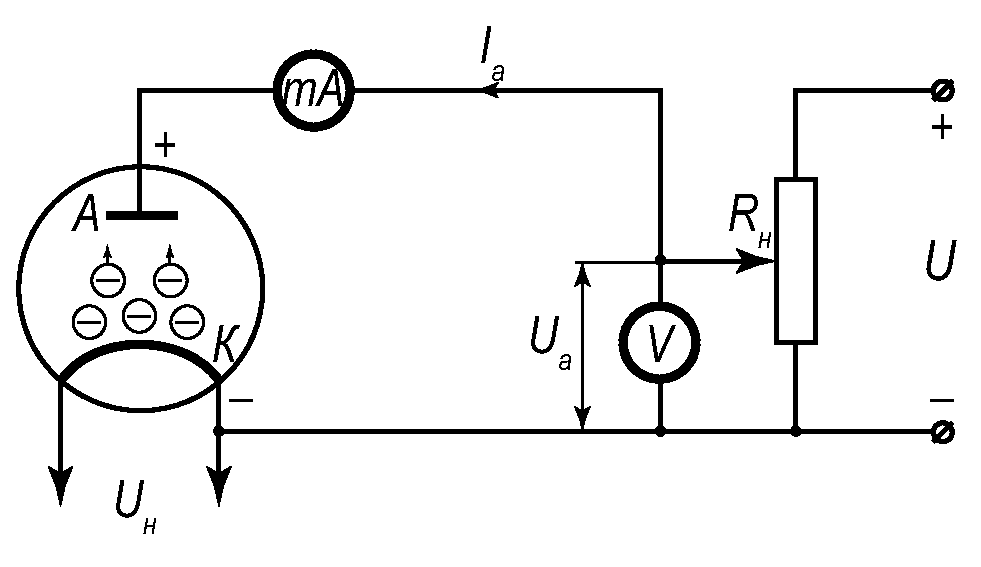
\includegraphics[width=\textwidth]{pic42}
		
	}
\caption{}
\label{pic42}
\end{figure}
%\end{center}

На рис. $\ref{pic42}$ показана схема вакуумной электронной лампы с двумя электродами — катодом и анодом. Здесь термоэлектронная эмиссия вызывается нагреванием катода электрическим током от источника напряжения накала $U_\text{н}$. Вылетевшие из катода электроны образуют электронное облако, электрическое поле которого налагается на поле, созданное электродами. Поле электронного облака будет препятствовать удалению вновь вылетающих электронов из катода. Поэтому часть их возвращается в металл. В конце концов создаётся динамическое равновесие между числом вылетающих из металла и возвращающихся в него электронов, напоминающее процесс, происходящий при наличии насыщенного пара над жидкостью.

Приложим теперь напряжение $U_\text{а}$ (называемое анодным) между анодом и катодом. Созданное в ваккуме электрическое поле заставит электроны двигаться к положительно заряженному аноду и через электронную лампу пойдёт ток $I_\text{a}$. По мере увеличения $U_\text{a}$ всё большее число электронов из объёмного заряда будет доходить до анода и величина $I_\text{a}$ будет расти. Наконец, наступит такое соотношение, при котором все электроны, испускаемые катодом, имеющим температуру $T$, долетают до анода, и объёмный заряд уничтожается. Дальнейшее увеличение анодного напряжения $U_\text{а}$ не влияет на силу анодного тока. Ток, сила которого не увеличивается с ростом напряжения, называется \emph{током насыщения} $I_\text{нас}$. По силе тока насыщения судят о числе электронов $N$, ежесекундно покидающих катод. Очевидно, что


\begin{equation}
N = \frac{I_\text{нас}}{e}.\nonumber
\end{equation}

\section{Вольтамперная характеристика}
Графически изображённая зависимость между силой тока и напряжением в данном приборе, называется вольтамперной характеристикой.

Изменяя анодное напряжение $U_\text{а}$ с помощью реостата $R_\text{н}$ (см. рис. 42) и измеряя это напряжение вольтметром, а анодный ток миллиамперметром, можно получить вольтамперную характеристику тока в вакууме (рис. 43). Вначале (пока лишь часть электронов достигает анода) анодный ток растёт благодаря отсасыванию электронов из объёмного заряда полем анода. Как показали американский инженер Лэнгмюр и московский физик Богуславский, зависимость $I_\text{a}$ от $U_\text{а}$ в начале характеристики выражается «законом трёх вторых»

\begin{equation}\label{zakon3/2}
I_\text{а} = \alpha U_\text{а}^{\frac{3}{2}}.
\end{equation}

Коэффициент пропорциональности $\alpha$ зависит от геометрических размеров, формы и взаимного расположения электродов и вычисляется или измеряется отдельно для каждой конструкции ламп.

Полукубическая парабола, уравнение которой дано формулой \ref{zakon3/2}, описывает рост анодного тока в функции от анодного напряжения на участке $Om_1$, $Om_2$.

Наибольшее значение анодного тока, получаемое при определенной температуре катода, и есть ток насыщения. Его величина зависит только от температуры, материала и величины поверхности катода. При повышении температуры ток насыщения быстро растёт (по показательному экспоненциальному закону).

Нижняя кривая на рис. 43 снята при температуре катода $T_1$, верхняя — при более низкой температуре $T_2$.

На рис. 44,\textit{а} показана опытная зависимость между током насыщения и температурой катода.

Теоретическая формула, связывающая ток насыщения, температуру катода и работу выхода электронов по энергиям согласно Ферми (см. лекцию 17) и называется формулой Ричардсона. Обычно формула Ричардсона приводится для плотности тока насыщения:
\begin{equation}
j_\text{нас} = \frac{I_\text{нас}}{S_\text{кат}} = BT^{2}e^{-\frac{A}{kT}}.
\end{equation}
Здесь $S_\text{кат}$ — площадь поверхности катода, $T$ — температура катода, $^{\circ}\text{ К}$, $A$ — работы выхода электронов из данного металла, $B$ — константа, равная для чистых металлов $1,2\cdot10^{6} \text{а/м}^{2}\cdot\text{град}$.

Увеличение тока насыщения может быть достигнуто, во-первых, уменьшением работы выхода (путём покрытия катода очень тонкий слоем тория, окиси бария) и, во-вторых, — увеличением температуры. Оба эти фактора сильно влияют на $I_\text{нас}$ благодаря наличию в формуле Ричардсона экспоненциального множителя. Так, повышение температуры вольфрамовой нити накала от $2000$ до $3000^{\circ}\text{ К}$, т. е. в полтора раза, увеличивает $I_\text{нас}$ в несколько миллионов раз.

На рис. 44, б изображена зависимость плотности тока насыщения (в логарифмическом масштабе) от величины, обратной температуре катода $(\frac{1}{T})$.


% Лекция 21
\chapter{Эмиссия электронов. Электронные приборы. Диод}
\section{Электронные приборы}
Двухэлектродная лампа — диод — представляет собой стеклянный или металлический баллон, в котором создан вакуум и впаяны два электрода — катод и анод. Диод используется в качестве выпрямителя и в качестве детектора электромагнитных колебаний в многочисленных радиотехнических и электротехнических устройствах. Выпрямляющий диод (кенотрон) пропускает ток, когда потенциал холодного электрода (анода) выше, чем горячего электрода (катода); при изменении знака разности потенциалов электрическое поле отбрасывает электроны назад, к горячему электроду, и ток через лампу не идёт (запирающее напряжение).

Если к диоду приложено переменное, например синусоидальное, напряжение, то он срезает отрицательные «полуволны» и создаёт импульсы тока (рис. 45,\textit{а} и 45,\textit{б}).

Для двухполупериодного выпрямителя используется двойной диод — лампа с одним катодом и двумя анодами (рис. 46). При этом в нагрузочном сопротивлении $R$ протекает пульсирующий ток (рис. 45,\textit{в}). 

Катод присоединяется к средней точке вторичной обмотки (точки \textit{1} и \textit{2}). Ток идёт через каждый анод только в течение одного полупериода. Пусть, например, полуволна переменного напряжения направлена сначала от \textit{2} к \textit{1}; ток пойдёт от точки \textit{1}, через первый анод $A_1$, на катод, через нагрузочное сопротивление $R$, в точку \textit{3} и вернётся в точку \textit{1}. В следующем полупериоде направление тока изменится — он будет протекать по обмотке трансформатора от \textit{1} к \textit{2}, на второй анод $A_2$, через катод, сопротивление $R$, в точки \textit{3} и \textit{2}.

В оба полупериода ток через сопротивление $R$ протекает в одном и том же направлении. Обмотка $T_\text{н}$ служит для питания цепи накала катода. Обычно пульсацию тока сглаживают путём зарядки и разрядки конденсатора, включаемого параллельно сопротивлению $R$ (на схеме не показан).

Для управления потоком электронов в лампе служит третий электрод — сетка, располагаемый между катодом и анодом. Сетка расположенная ближе к катоду, чем анод, и её потенциал сильнее влияет на анодный ток, чем потенциал анода.

Действительно, для создания у катода одинаковой напряжённости электрического поля $E$ на более далёкий анод надо подавать более высокое напряжение, чем на сетку. Вспомнив, что напряжённость электрического поля равна градиенту потенциала\begin{equation}
E = \frac{\Delta U}{\Delta l}\nonumber
\end{equation} и обозначив расстояние от катода до сетки $\Delta l_c$, а до анода $\Delta l_a$, получаем, что при одинаковом E\begin{equation}
\Delta U_c = -E\Delta l_c,\nonumber
\end{equation} а \begin{equation}
\Delta U_a = -E\Delta l_a.\nonumber
\end{equation}

Так как $\Delta l_a>\Delta l_c$, то по абсолютному значению $\Delta U_a>\Delta U_c$. Величина плотности анодного тока $j_a$ в лампе зависит от напряжённости поля, созданного потенциалами анода и сетки; рост $E$ вызывает увеличение плотности тока.

Лампа с сеткой — триод служит для усиления малых напряжений. На рис. 47 изображена схема включения триода (источник тока для накала катода обычно не показывается).

Сеточная характеристика триода, т. е. зависимость анодного тока $I_a$ от напряжения на сетке $U_c$, показана на рис. 48. Здесь изображены две сеточные характеристики, снятые при различных напряжениях на аноде $(U_a2>U_a1)$.

При отсутствии напряжения на сетке анодный ток создаётся анодным напряжением. Для того чтобы $I_a=0$, необходимо приложить к сетке отрицательное запирающее напряжение $U_\text{зап}$. Обычно на сетку подаётся некоторое отрицательное напряжение, называемое начальным смещением $U_{c_0}$.

Если на сетку подавать малые изменения напряжения $\Delta U_c$, то они вызовут изменения анодного тока на величину $\Delta l_a$; при этом на большом нагрузочном сопротивлении произойдёт падение напряжения $\Delta U_a=R_\text{н} \Delta I_a$, б$\acute{\text{о}}$льшее, чем $\Delta U_c$. В этом состоит усилительное действие лампы.

Триод принято характеризовать тремя параметрами: крутизной характеристики $S$, коэффициентом усиления $\mu$ и внутренним сопротивлением $R_i$.

Рассмотрим треугольник $abc$ на прямолинейном участке сеточной характеристики (рис. 48).

Отношение приращения анодного тока $\Delta I_a$ к вызвавшему его изменению сеточного напряжения $\Delta U_c$ при неизменном напряжении на аноде (например, $U_{a_2}$), называют крутизной характеристики
\begin{equation}
S = (\frac{\Delta I_a}{\Delta U_c})_{U_a=const}.
\end{equation}

Отношение приращения анодного напряжения $\Delta U_a$ к изменению сеточного напряжения $\Delta U_c$, при котором анодный ток остаётся постоянным, называется статическим коэффициентом усиления триода $\mu$ \begin{equation}\label{mu_21.2}
\mu = - (\frac{\Delta U_a}{\Delta U_c})_{I_a=const}.
\end{equation}

Для сохранения анодного тока неизменным надо, например, увеличить анодное напряжение $(\Delta U_a > 0)$) и уменьшить потенциал сетки $(\Delta U_c < 0)$. Поэтому в формуле \ref{mu_21.2} стоит знак минус, т. е сама величина $\mu$ положительна. Можно дать следующее простое определение важнейшего параметра триода — коэффициента усиления $\mu$: величина $\mu$ показывает, во сколько раз сеточное напряжение сильнее влияет на анодный ток, чем анодное.

Внутренним сопротивлением лампы $R_i$ называют отношение приращения анодного напряжения $\Delta U_a$ к вызванному им приросту анодного тока $\Delta I_a$ при постоянном сеточном напряжении\begin{equation}\label{21.3}
R_i = (\frac{\Delta U_a}{\Delta I_a})_{U_c=const},
\end{equation}
причём $\Delta U_a = U_{a_2}-U_{a_1}$, т. е. рассматриваются две сеточные характеристики при различных анодных напряжениях и постоянном $U_c$. Легко показать, что\begin{equation}\label{21.4}
\frac{S R_i}{\mu} = 1.
\end{equation}

Действительно, \begin{equation}
\frac{\frac{\Delta I_a}{\Delta U_c}\cdot\frac{\Delta U_a}{\Delta I_a}}{\frac{\Delta U_a}{\Delta U_c}} = 1.\nonumber
\end{equation}

Соотношение \ref{21.4} называется уравнением Баркгаузена.

Для ламп с одной сеткой величина $\mu \approx 10 \div 15$. Для большего усиления напряжение, снятое с сопротивления $R_\text{н}$, подаётся на сетку следующей лампы (второй каскад усиления), и т. д. Кроме этого, в лампу можно ввести вторую, третью сетки, повысив этим $\mu$ до $100 \div 1000$.

\section{Умножители. Вторичная электронная эмиссия}

При ударе электронов и ионов о металлы и полупроводники происходит выбивание электронов из твёрдых веществ, т. е. имеет мето так называемая вторичная электронная эмиссия. Коэффициентом вторичной электронной эмиссии $\delta$ назовём отношение числа выбитых вторичных электронов $N_2$ к числу первичных падающих $N_1$.

\begin{equation}
\delta = \frac{N_2}{N_1}.
\end{equation}

Этот коэффициент для металлов колеблется от 1,25 (Ni) до 1,78 (Pt), а для полупроводников достигает значения 10 и более.

На описанном явлении основано действие так называемых умножителей, разработанных Кубецким, Векшинским и другими учёными.

Рассмотрим фотоэлектронный умножитель (ФЭУ), рис. 49. При освещении первого катода слабым пучком света из него благодаря фотоэффекту вырываются электроны. Проследим за движением одного из них. Ускоряясь в поле с разностью потенциалов $U$ между первым и вторым катодом, этот электрон выбивает из второго катода $\delta$ электронов. Пролетая от второго катода к третьему, электроны снова ускоряются той же разностью потенциалов и выбивают уже $\delta\cdot\delta=\delta^{2}$ электронов. При наличии $n$ электродов в умножителе число вылетевших их последнего катода электронов больше числа вырванных их первого в $\delta^{n-1}$ раз.

ФЭУ гашли широкое применение для усиления слабых фототоков, например для счёта частиц в ядерной физике.

\section{Автоэлектронная эмиссия}

Если создать в вакууме сильное электрическое поле, прикладывая между катодом и анодом напряжение поряжка нескольких тысяч вольт, то из холодного катода, выполненного в форме острия, начнут вырываться электроны.

Явление вырывания электронов из холодного катода сильным электрическим полем называется автоэлектронной эмиссией. Наибольший градиент потенциала\begin{equation}
E = \frac{\mathbf{d}U}{\mathbf{d}r}
\end{equation} получается как раз вблизи катода. При радиусе кривизны острия $r=10^{-6} \textit{ м} = 1 \textit{ мкм} $ и разности потенциалов в трубке, равной 1000 $\textit{в}$, напряжённость поля у катода достигает громадной величины — $10^(8)\textit{ в/м} $.

При автоэлектронной эмиссии работа выхода в значительной мере преодолевается за счёт работы, совершаемой над электронами сильным внешним электрическим полем.

Явление автоэлектронной эмиссии играет исключительно важную роль при образовании и поддержании электрической дуги (см. лекцию 24).

% Лекция 22
\chapter{Ток в электролитах}

Электролитами, или проводниками второго рода, называют вещества с ионной проводимостью, а именно растворы солей, щелочей и кислот, а также расплавы солей. Прохождение тока через электролиты связано с переносом вещества, отложением его на электродах и с химическими изменениями. Этим электролиты отличаются от проводников первого рода, например металлов, где ток не вызывает переноса вещества и химических процессов. Ионной проводимостью обладают не только жидкие электролиты, но и некоторые ионные кристаллы.

А. Ф. Иоффе изучил явление электролиза у кристаллов NaCl. Металлический натрий перемещается внутри кристаллической решётки и образует ветви, распространяющиеся в кристалле от электрода. Ионная проводимость обнаружена и у многих полупроводников. При повышении температуры сопротивление ионных кристаллов падает, как и у обычных электролитов.

Как известно, при растворении солей, кислот и щелочей их молекулы распадаются на заряженные частицы — ионы. Это связано с тем, что на электрические силы притяжения между ионами налагаются противоположные по направлению силы со стороны поляризованных молекул растворителя, ориентированных полем ионов (рис. 50). Формально это происходит так, как будто сила электрического притяжения, действующая между ионами в молекуле, уменьшается в $\epsilon$ раз. Величина диэлектрической проницаемости $\epsilon$ у воды достигает 81. Значительное убывание силы взаимодействия приводит к тому, что энергия теплового движения частиц жидкости становится достаточной для разрушения молекул. Распад молекул данного вещества на ионы при растворении называется $\emph{электролитической диссоциацией}$. Степень диссоциации характеризуется коэффициентом диссоциации $\alpha$. Это число, указывающее, какая доля общего количества молекул электролита распалась на ионы. Величина $\alpha$ зависит от рода вещества и увеличивается при нагревании. Если концентрация нейтральных молекул в растворе $n_0$, а коэффициент диссоциации $\alpha$, то концентрация ионов будет $\alpha\cdot n_0$. При $\alpha=0$ диссоциация отсутствует; $\alpha=1$ соответствует диссоциации всех молекул. Последнее имеет место в сильно разбавленных электролитах, где ионы противоположных знаков редко встречаются друг с другом.

При диссоциации происходит разделение зарядов ранее нейтральных молекул, поэтому общий заряд в единице объёма электролита равен нулю. Вследствие этого при одинаковой валентности концентрация положительных ионов $n_+$ будет равна концентрации отрицательных ионов $n_-$\begin{equation}\label{22.1}
n_+ = n_- = \alpha\cdot n_0.
\end{equation}

Если валентность ионов $Z$, то заряд каждого из них равен $Ze$, где $e$ — заряд электрона.

\begin{equation}\label{22.2}
q_{0+} = q_{0-}- = Ze.
\end{equation}

Если в объёме электролита создать электрическое поле напряжённости $E$, подключив к опущенным в раствор электродам постоянное напряжение $U$, то силы, действующие на ионы разного знака, начнут перемещать их в противоположных направлениях, что и создаст ток в электролите. Применим формулу $\ref{159}$ к ионному току. Носителями тока в жидкостях являются положительные и отрицательные ионы\begin{equation*}
j = (n_+ q_{0+} u_+ + n_- q_{0-} u_-)E.
\end{equation*}

Учитывая выражения $\ref{22.1}$ и $\ref{22.2}$, получим следующую формулу для закона Ома в электролитах:

\begin{equation}\label{22.3}
j = \alpha n_0 Ze (u_+ + u_-)E.
\end{equation}

Электропроводность электролитов $\gamma$ выразится как\begin{equation}\label{22.4}
\gamma = \alpha n_0 Ze (u_+ + u_-).
\end{equation}

Вспоминая, что подвижность ионов $u=\frac{q_0}{6\pi \eta r}$, где $\eta$ — коэффициент вязкости, видим, что при нагревании электролита подвижность растёт вследствие падения вязкости; одновременно при нагревании увеличивается коэффициент диссоциации. Следовательно, при повышении температуры электропроводность электролитов заметно растёт.

\section{Закон Фарадея}

В 1836 году Фарадей на опыте установил, что масса вещества, выделившегося при электролизе на катоде или аноде, зависит от рода вещества и пропорциональна количеству электричества, протекшего через электролит. Допустим, что на электроде выделилась масса вещества $M$. Очевидно, что если $m$ — масса каждого иона, а $N$ их число, то \begin{equation*}
M=mN.
\end{equation*}

Масса каждого иона $m=\frac{A}{N_0}$, где $A$ — масса $\textit{кг-атома}$, а $N_0$ — число Авогадро.

Число ионов $N$ равно общему заряду, прошедшему через электролит $q$, делённому на заряд одного иона $Ze$ ($Z$ — валентность иона)\begin{equation*}
N=\frac{q}{Ze}.
\end{equation*}

Следовательно, \begin{equation*}
M=\frac{A}{N_0}\frac{q}{Ze} = \frac{A}{Z}\frac{1}{N_0 e}q.
\end{equation*}

В этой формуле произведениее $N_0 = F$ — общий заряд $\textit{кг-экв}$ атомов данного вещества. Эта величина называется числом Фарадея\begin{equation*}
F=6,02\cdot10^{26}\cdot1,6\cdot10^{-19} = 9,654 \cdot 10^7  \frac{\textit{к}}{\textit{кг}\cdot\textit{экв}}.
\end{equation*}

Окончательно получаем объединённый закон Фарадея в следующем виде: \begin{equation}\label{22.5}
M = \frac{1}{F}\cdot\frac{A}{Z}\cdot q,
\end{equation} т. е. масса вещества, выделившегося при электролизе, пропорциональна массе $\textit{кг-атома}$ и количеству электричества, протёкшего через электролит, и обратно пропорциональна валентности вещества.

Соотношение между — числом Авогадро $N_0$, величиной элементарного заряда $e$ и числом Фарадея $F$ — даёт возможность по двум из них найти третью. Например, $e = \frac{F}{N_0}$, а $N_0 = \frac{F}{e}$.

В физике были использованы обе возможности. Число Авогадро было определено из опытов с броуновским движением (опыты Перрена), и это позволило найти заряд электрона $e$. после точного измерения заряда электрона в опытах Милликена оказалось возможным определить число Авогадро.

\section{Применение электролиза}

Из школьного курса физики известно, что электролиз применяется для получения чистых металлов (алюминия, магния) из расплавленных солей, для покрытия поверхностей металлических предметов слоем других металлов, получения изображения (матрицы) различных предметов электролитическим путём. За последние 20 лет получили распространение электролитические методы обработки металлов, разработанные в СССР — электрополировка, катодно-механическая резка металлов.

Как известно, наибольшая напряжённость поля имеется вблизи выступающих участков поверхности проводника, а у вогнутых участков она минимальна. Плотность тока пропорциональна напряжённости и также максимальна у выступающих участков. Если полируемое металлическое изделие сделать анодом, то при электролизе сильнее всего будет растворяться выступающие участки, что приводит к сглаживанию, полировке изделия. Электрополировка применяется при обработке таких ответственных деталей, как лопасти турбин и др.

При анодно-механическое резке металлов обрабатываемая деталь служит анодом. Вращающийся железный или медный диск с тонкими краями является катодом; он прижимается к изделию и смачивается специальным электролитом. В тех местах, где диск приближается к изделию, плотность тока наибольшая и происходит быстрое удаление металла, изделие «режется» диском. В этом процессе существенную роль играют также химические, тепловые и механические воздействия.

% Лекция 23
\chapter{Газовый разряд}

Газы состоят их нейтральных молекул и являются хорошими изоляторами. Изоляционные свойства воздуха широко используются в электротехнике и связи: так, в линиях электропередач ток высокого напряжения идёт по голым проводам, надземные телеграфные и телефонные линии также осуществляются проводами без изоляции.

Однако ещё в конце XVIII века Кулон обнаружил, что заряженный и укреплённый на хорошо изолирующей подставке электроскоп через некоторое время разряжается. Впоследствии было замечено, что разрядка электроскопа идёт быстрее, чем это могло бы быть вызвано утечкой тока через подставку. Отсюда можно было сделать вывод, что в газах под действием каких-то причин создаются заряженные частицы.

Процесс разделения нейтральной молекулы газа на электрон и положительный остаток — ион — носит название $\emph{ионизации}$.

Отрыв электрона от нейтральной молекулы, т. е. ионизация, вызывается внешними факторами, называемыми ионизаторами. Способностью ионизировать газы обладают: космические лучи, $\alpha$-, $\beta$- и $\gamma$-лучи, испускаемые радиоактивными веществами; лучи Рентгена; ультрафиолетовые лучи; источники высокой температуры (например, пламя); быстрые электроны и ионы, разогнанные электрическим полем.

При ионизации наряду с положительными ионами образуются и отрицательные, так как свободные электроны иногда <<захватываются>> полем ядер и атомов, образующих молекулу. Молекула с <<прилипшим>> к ней электроном и является отрицательным ионом. Из сказанного следует, что носителями тока в газах являются положительные и отрицательные ионы и электроны. 

Наряду с процессом ионизации в газе происходит обратный процесс -- восстановление нейтральных молекул из электронов и ионов. Это явление называется $\emph{рекомбинацией}$, или молизацией.

Если в объёме ионизированного газа создать электрическое поле, то на тепловое хаотическое движение ионов и электронов наложится направленное перемещение -- пойдёт ток. Прохождение тока через предварительно ионизированный газ называется $\emph{несамостоятельным разрядом}$. Прохождение тока через газ без внешнего ионизатора называется $\emph{самостоятельным разрядом}$.

\section{Основные количественные соотношения в газовом разряде}

При прохождении тока через газ ионы, создаваемые ионизатором, частично доходят до электродов и там нейтрализуются.

Обозначим число ионов, создаваемых в 1$\textit{ сек}$ в единице объёма газа под действием ионизаторов, через $n_0$, число ионов, рекомбинирующих в единице обёма в 1$\textit{ сек}$, -- $n'$,  а число ионов, в 1$\textit{ сек}$ уходящих из единицы объёма на электроды и нейтрализующихся там, - $n''$. Нейтрализация состоит в том, что положительные ионы, попадая на катод, получают от него электроны, а отрицательные ионы отдают лишний электрон на аноде.

В начале действия ионизатор число ионов в газе возрастает, но через некоторое время наступает равновесие между количеством ионов, создаваемых и уничтожающихся в результата рекомбинации и нейтрализации.

Для установившегося процесса можно написать следующее равенство:
\begin{equation}\label{23.1}
n_0 = n' + n''.
\end{equation}

В единице объёма газа при данной силе тока будет находиться некотрое <<равновесное>> количество ионов $n$.

Считая концентрацию ионов обоих знаков одинаковой, легко получить выражение для числа рекомбинирующих ионов $n'$. Очевидно, $n'$ будет пропорционально произведнднию концентрации положитедльных и отрицательынх ионов, т. е.\begin{equation}\label{23.2}
n' = \alpha n n = \alpha n^2.
\end{equation}

Коэффициент пропорциональности $\alpha$ -- это коэффициент рекомбинации, зависящий от рода ионов, давления, температуры. При увеличении температуры $\alpha$ возрастает, так как растёт число столкновений; повышение давления вызывает уменьшение $\alpha$, так как возрастает концентрация нейтральных частиц газа, что уменьшает вероятность встречи ионов разного знака.

Если за время $t$ к пластинам (электродам) через объём газа $S\cdot L=V$ перенесён общий заряд $q$, то общее число нейтрализующихся ионов равно частному $\frac{q}{q_0}$, где $q_0$ -- заряд каждого иона. Число $n''$ ионов, нейтрализующихся за 1$\textit{ сек}$ из единицы объёма, найдётся из соотношения \begin{equation}\label{23.3}
	n'' = \frac{q}{q_0 tV} = \frac{I}{q_0 V},
\end{equation}где $I = \frac{q}{t}$ -- сила тока, проходящего через газ.

Подставляя в формулу $\ref{23.1}$ выражения для $n'$ и $n''$, получим
\begin{equation}\label{23.4}
n_0 = \alpha n^2 + \frac{I}{q_0 V}.
\end{equation}

Рассмотрим теперь два крайних случая.

1. Напряжение между электродами и сила тока $I$ весьма малы. Это означает, что подавляющая часть ионов рекомбинирует и до пластин доходит ничтожное количество, т. е. $n'' \ll n'$. В этом случае равновесная концентрация будет наибольшей. Тогда из $\ref{23.4}$ получаем:
\begin{equation}\label{23.4a}
n_0 \approx \alpha n^2.
\end{equation}

Это соотношение даёт возможность приближённо определить величину $\alpha$ по $n_0$ и наибольшему значению $n$.

2. При увеличении напряжения скорость ионов возрастает, они быстрее пролетают между электродами и вероятность рекомбинации сильно уменьшается. Основная масса ионов, создаваемых ионизатором, доходит до пластин, где и нейтрализуется. Теперь $n' \ll n''$. В этом случае формула $\ref{23.4}$ даёт соотношение\begin{equation}\label{23.5}
n_0 \approx \frac{I}{q_0 V},
\end{equation}означающее, что дальнейший рост напряжения не вызывает увеличения тока, так как практически все ионы, создаваемые ионизатором, доходят до пластин.

Ток в газе, сила которого $I$ не зависит от напряжения, называется током насыщения \begin{equation}\label{23.5a}
I_{\text{нас}} = n_0 q_0 V.
\end{equation}


Величина тока насыщения зависит только от интенсивности ионизатора $n_0$ и объёма газа $V$.

При дальнейшем увеличении напряжения наступает ионизация ударом. Электроны, разогнанные полем на длине свободного пробега $\lambda$, приобретают кинетическую энергию $W_{\text{к}}$, достаточную для отрыва электрона от нейтральной молекулы. Работа, которою нужно совершить для отцепления электрона от данного атома или молекулы, называют $\emph{работой ионизации}$ $А_i$.

Величина\begin{equation*}
\frac{А_i}{e} = U_i
\end{equation*} носит название $\emph{потенциала ионизации}$.

$U_i$ -- это разность потенциалов, при прохождении которой электрон приобретает энергию, достаточную для ионизации.

Для ионизации ударом необходимо, чтобы\begin{equation}\label{23.6}
W_k \ge А_i.
\end{equation}

Электрон приобретает энергию, разгоняясь в электрическом поле напряженности $E$ на пути между двумя столкновениями, т. е. на расстоянии $\lambda$. Разность потенциалов, которую пролетает электрон, $U_{\lambda}$, связана с $E$ и $\lambda$ известным соотношением\begin{equation*}
U_{\lambda} = E \lambda_E,
\end{equation*}где $\lambda_E$ -- проекция $\lambda$ на направление поля.

Для возникновения ударной ионизации должно быть\begin{equation}\label{23.7}
U_{\lambda} \ge U_i,
\end{equation}
или
\begin{equation}\label{23.8}
e \lambda_E E \ge A_i.
\end{equation}

При ионизации столкновением происходит <<неупругий>> удар электрона об атом или молекулу. Так как масса электрона в тысячи раз меньше массы частиц, с которыми он сталкивается, то как следует из теории удара, электрон может истратить практически всю своб кинетическую энергию на ионизацию. Если же с нейтральной молекулой сталкивается разогнанный в поле ион, то благодаря его большой массе значительная часть его кинетической энергии расходуется на увеличение скорости нейтральной частицы (см. раздел механики), что затрудняет ионизацию. Кроме того, у электрона благодаря меньшему, чем у иона, диаметру, длина свободного пробега больше, и согласно формуле $\ref{23.8}$ электроны между столкновениями приобретают в поле большую энергию, чем ионы.

При ионизации ударом ток в газе с ростом напряжения начинает возрастать все значительнее, так как при этом заметно увеличиваются число электронов и ионов. Новые электроны также разгоняются и ионизируют всё большее число молекул. При достаточно больших разностях потенциалов ионизацию ударом производят также ионы.

\section{Вольтамперная характеристика разряда}

Рассмотрим результаты опытного изучения несамостоятельного разряда в газах. Для этого обратимся к схеме, изображенной на рис. 51. Газ, находящийся между двумя металлическими пластинами -- анодом и катодом, подвергается действию ионизатора постоянной интенсивности. Изменяя напряжение $U$, приложенное к пластинам, измеряют его величину и силу тока в цепи. Оказывается, что последняя будет изменяться так, как это показано на рис. 52, где изображена вольтамперная характеристика несамостоятельного разряда в газе.

Как видно, сила тока, приблизительно пропорциональна напряжению лишь при малых значениях $U$; таким образом, закон Ома в газах выполняется только при небольших электрических полях (участок $Оа$); затем (участок $ab$) ток меняется уже не по закону Ома, величина его отстает от линейной зависимости (изображена пунктиром). При дальнейшем увеличении напряжения сила тока остается почти постоянной (участок $bc$); затем ток снова растёт, причём его увеличение становится всё более резким (участки $cd$ и $de$). Оказывается, что участок $bc$ характеризует состояние насыщения, рассмотренное в лекции 23.

Когда электроны приобретают энергию, достаточную для совершения работы ионизации, происходит ударная ионизация ($cd$), в результате которой ток сильно возрастает. Действительно, электрон, совершивший ионизацию ударом, и электрон, выбитый им из молекулы, разогнавшись в поле, ионизируют еще две молекулы. Теперь получатся уже четыре электрона, которые также могут совершить ионизацию ударом, и т. д.

Таким образом, после $n$ свободных пробегов, заканчивающихся ионизацией ударом, число получившихся электронов (и положительных ионов) будет равно $2^n$. Этим и объясняется создание лавины, которая, как показали исследования тока в газе, перемещается от катода к аноду со скоростью около $10^5 \textit{м/сек}$ (см. уча. сток $de$).

% Лекция 24
\chapter{Газовый разряд (окончание)}
\section{Самостоятельный разряд}
Следует заметить, что образования лавины ещё недостаточно для возникновения самостоятельного разряда. Последний вызывается вырыванием новых электронов из катода. Для возникновения самостоятельного разряда в газе количество создаваемых электронов и ионов должно превышать их убыль.

Вырывание электронов из катода может быть результатом нескольких процессов: электроны могут выбиваться из катода положительными ионами или вырываться квантами света, испускаемыми светящимся при разряде газом (фотоэффект) — при ударе электронов о молекулы или атомы газа может происходить процесс возбуждения, т. е. электроны в этих частицах «забрасываются» на более высокие энергетические уровни, при возврате электронов на нормальные уровни атомы испускают свет.

Процесс перехода разряда из несамостоятельного в самостоятельный происходит при напряжении, называемом напряжением зажигания, или пробоя $U_\text{з}$. Опытами установлено, что это напряжение зависит от произведения $pl$, где $р$ — давление газа, а $l$ -- расстояние между электродами. Это значит, что если $р$ увеличить, а  уменьшить во столько же раз, то $U_\text{з}$ не изменится. При достаточно больших значениях произведения $pl$ величина $U_\text{з}$ растёт почти пропорционально этому произведению.

Для получения самостоятельного разряда при неизменном $l$ можно поступить двояко:
1)	при постоянном напряжении между электродами уменьшить давление; при этом длина свободного пробега электронов увеличится обратно пропорционально давлению и создадутся условия для ионизации ударом;
2)	при неизменном давлении увеличить напряженность $Е$ электрического поля в газе путем повышения напряжения между электродами (напомним, что $Е = -\frac{\mathbf{d}U}{\mathbf{d}l}$).

Различают следующие виды самостоятельного разряда в газах: искровой, тлеющий и дуговой.

\section{Искровой разряд. Корона}

Если газ находится при атмосферном давлении, то самостоятельный разряд возможен только при очень высоком напряжении на электродах, когда даже на малых длинах свободного пробега электроны приобретают кинетическую энергию, достаточную для ионизации ударом [см. формулу $\ref{23.8}$].

При больших энергиях электронов, приобретенных в сильных полях, вырывание электронов при столкновении возможно не только из внешних, но и из внутренних слоёв, близких к ядру в молекулах (атомах) газа. Когда на освободившиеся места переходят электроны с внешних слоев, то происходит испускание ультрафиолетовых и даже рентгеновских лучей, являющихся ионизаторами и создающих электроны и ионы во всем объёме газа. Так возникают новые электронные лавины, сосредоточенные в канале малого сечения сильно ионизированного газа — так называемые стримеры. Они с большой скоростью ($\sim 10^6 \textit{м/сек}$) передвигаются от области с наибольшей концентрацией электронных лавин — анода — к катоду.

Когда стримеры достигают катода, то цепь замыкается — между пластинами в газе проскакивает искра, представляющая собой тонкий шнур с ветвями. Искра состоит из сильно ионизированного газа; так как сопротивление тонкого искрового канала мало, то сила тока в цепи сильно возрастает и напряжение на зажимах источника резко падает. В искре выделяется большое количество тепла и газ начинает ярко светиться. Нагрев сопровождается резким повышением давления, создаются механические ударные и звуковые волны (этим объясняется гром при искровом разряде — молнии).


Как известно из электростатики, напряженность поля (градиент потенциала) у острия достигает очень больших значений; следовательно, вблизи острия имеется сильная ударная ионизация. При этом электроны возбуждают молекулы газа ударом и область газа вблизи острия сильно светится — наблюдается коронный разряд, или корона.

Большую величину градиента потенциала у острия можно продемонстрировать следующим опытом:

Если изогнуть укрепленную на оси металлическую проволоку в виде буквы Z и концы её заострить, то при подведении к такому проводнику напряжения порядка $10^3 \div 10^4 \textit{в}$, он начнет вращаться в сторону, противоположную заострениям. Это объясняется тем, что ионы, имеющие заряд того же знака, что и острие, будут отталкиваться от него и приведут проволоку во вращение.

\section{Тлеющий разряд}

Для получения тлеющего разряда в газе надо создать разрежение. К электродам, впаянным в достаточно длинную стеклянную трубку, подводится напряжение порядка $10^3 \textit{в}$. При атмосферном давлении разряда нет. Если начать откачивать воздух из трубки с помощью насоса, через трубку пойдёт слабый ток. При давленна порядка $130 \textit{ н/м}^2$ ($1\textit{ мм рт. ст.}$) газ начнет светиться, причём цвет свечения зависит от химического состава газа. Такое свечение газа в трубках с разреженным неоном, аргоном, парами ртути широко используется для различных световых надписей, реклам.

При дальнейшем уменьшении давления до $10 -- 15 \textit{ н/м}^2$ ($0,01\textit{ мм рт. ст.}$ средняя и прилегающая к аноду часть светящегося столба газа разбивается на отдельные участки — страты.

При увеличении разрежения ток убывает, свечение газа прекращается. Наблюдается зеленоватое свечение стекла против катода.

Слабый ток в начале откачки газа объясняется тем, что имеющееся в трубке небольшое число положительных ионов приобретает на возросшей благодаря понижению давления длине свободного пробега энергию, достаточную для выбивания из катода электронов при ударе. При столкновениях с молекулами газа электроны, разогнанные в электрическом поле, могут возбуждать молекулы газа, что вызывает свечение. Большая часть столкновений не вызывает ударной ионизации. При дальнейшей откачке доля столкновений, приводящих к ударной ионизации, возрастает, но ток растет незначительно, так как концентрация заряженных частиц при малом давлении мала. При увеличении разрежения концентрация падает, электроны и ионы уже почти не сталкиваются с молекулами; этим и объясняется убывание тока и прекращение свечения. Быстрые электроны, ударяясь о стекло против катода, вызывают его флюоресценцию.

Важную роль в тлеющем разряде играет катодное падение потенциала. Вблизи катода плотность объемного заряда положительных ионов велика; в прикатодной области эти ионы приобретают значительную энергию и здесь же разгоняются электроны, вырванные ударами ионов из катода. В прикатодном слое происходит значительная ударная ионизация молекул электронами.

Благодаря большому падению потенциала вблизи катода напряженность поля в этой области достигает значительной величины.

\section{Дуговой разряд}

В начале ХIХ века Петров и Дэви, независимо друг от друга, открыли дуговой разряд, часто называемый дугой. Если приложить напряжение к соприкасающимся угольным электродам, а затем развести их, то благодаря быстрому возникновению большой плотности тока на небольшом участке катода угли раскаляются и между ними возникает ослепительное пламя. Температура в дуге достигает $4000^{\circ}$ С при атмосферном давлении, а при повышенном давлении газа до $15 000^{\circ}$ С. При разведении электродов сопротивление промежутков между ними сравнительно велико и в дуге начинает выделяться значительное количество тепла; газ между электродами сильно ионизируется. При этом сопротивление падает и далее дуга «горит» при уменьшенном по сравнению с начальным напряжении (всего в несколько десятков вольт).

Плотность тока в дуге может достигать $10\textit{ а/мм}^2 = 10^7\textit{ а/м}^2$ и 6олее. Постепенно угольные электроды дуги сгорают — уголь соединяется с кислородом воздуха и на аноде образуется впадина, называемая кратером.

Высокотемпературная угольная дуга используется для плавки металлов, при дуговой электросварке и в мощных прожекторах для освещения. Разряд можно получить и с металлическими электродами.

Через сто лет после открытия дуги В. Ф. Миткевич объяснил механизм её «горения». Оказалось, что основной причиной, создающей и поддерживающей дугу, является испускание электронов из катода, раскаляемого ударами положительных ионов.

Если создать дугу при пониженном давлении, то ионизированный газ между электродами будет холодным вследствие малой концентрации ионов. Такая «холодная» дуга используется для выпрямления переменного тока в ртутном выпрямителе и как источник ультрафиолетовых лучей в ртутной лампе. Источником электронов в ртутной дуге служит катодное пятно — небольшой участок на поверхности ртути. Благодаря катодному падению потенциала плотность тока вблизи катодного пятна достигает огромных значений: $10^{12}\textit{ а/м}^2 = 10^6\textit{ а/мм}^2$ ; при этом электроны «вытягиваются» сильным электрическим полем из катода, т. е. происходит автоэлектронная эмиссия (см. лекцию 21).

\section{Плазма}

Сильно ионизированное вещество с суммарным объемным зарядом, равным нулю, обладает свойствами, резко отличными от свойств известных трех агрегатных состояний вещества; твердого, жидкого и газообразного. Такое состояние получило название четвертого агрегатного состояния, или плазмы.

При очень большой плотности тока в газе происходит почти полная ионизация его молекул и атомов. Такой газ состоит из электронов и положительных ионов, обладающих очень большими скоростями, и называется низкотемпературной (газоразрядной) плазмой. Сопротивление её весьма невелико, так как концентрация ионов значительна, нейтральных частиц мало, кроме того, в плазме содержатся однократно- и многократно-ионизированные частицы.

Высокотемпературная плазма является основным агрегатным состоянием глубинных областей Солнца и других звезд. Там температуры достигают десятков миллионов градусов, а давление — миллиардов атмосфер. Атомы газа полностью ионизированы, т. е. распались на электроны и ядра.

Убыль ионов, вызываемая рекомбинацией, в низкотемпературной плазме пополняется благодаря ионизации ударом, а в высокотемпературной плазме — столкновениями частиц, имеющих громадные скорости теплового движения.

В настоящее время уже в лабораторных условиях в плазме, в которой происходит электрический разряд большой мощности, получены на весьма короткие промежутки времени температуры в миллионы градусов. Заряженные частицы плазмы удерживаются в данном объеме магнитным полем, созданным сильным током, протекающим через плазму.

Перспективы использования ядерной энергии в управляемых термоядерных реакциях связаны с исследованиями высокотемпературной плазмы.

% Лекция 25
\chapter{Полупроводники}
\section{Основные особенности полупроводников}

По величине удельного электрического сопротивления $\varrho$ твердые тела можно разделить на проводники (металлы), у которых\begin{equation*}
\rho = \frac{1}{\gamma} = 10^{-8} \div 10^{-6} \textit{ ом • м},
\end{equation*}
полупроводники\begin{equation*}
\rho = \frac{1}{\gamma} = 10^{-6} \div 10^{3} \textit{ ом • м},
\end{equation*}
и изоляторы
\begin{equation*}
\rho = \frac{1}{\gamma} = 10^{3} \div 10^{16} \textit{ ом • м},
\end{equation*}

Важной особенностью полупроводников является сильная зависимость их свойств, в первую очередь сопротивления, от внешних воздействий: нагрева, деформации, облучения светом, рентгеновским н ядерным излучением.

Как показали экспериментальные исследования, зависимость дельной электропроводности $\gamma_T$ полупроводников от температуры $T$ довольно хорошо описывается формулой\begin{equation}\label{25.1}
\gamma_T = \gamma_0 e^{-\frac{b}{T}},
\end{equation}
где $\gamma_0$ и $b$ -- постоянные величины, значение которых выяснено ниже.

Увеличение температуры вызывет сильный рост электропроводности полупроводников в отличие от металлов, у которых $\gamma$ с повышением температуры убывает\begin{equation*}
\gamma_t = \frac{\gamma_0}{1+\alpha t}.
\end{equation*}

Установление температурной зависимости проводимости или сопротивления является самым надежным способом, позволяющим отличить полупроводниковую проводимость от металлической, в особенности, если это затруднительно сделать по абсолютному значению этих величин. К полупроводникам относятся некоторые элементы из средней части таблицы Менделеева — кремний (Si) , германий (Ge), селен (Se), углерод — алмаз (C), теллур (Te), олово (Sn) в серой модификации, кристаллическая сера (S) и др. Полупроводниками являются также окислы некоторых металлов  Cu$_2$O, ZnO, MgO, TiO$_2$, UO$_2$ и др., сульфиды PbS, CdS, AgS, ионные  кристаллы солей — KCl, NaCl, соединения PbSe, РЬТе. За последнее время получили распространение полупроводниковые соединения элементов третьей группы с элементами пятой группы таблицы Менделеева (вида А$_3$В$_5$), соединения вида А$_2$В$_4$.

Изучение свойств полупроводников и внедрение их в различные области техники началось с конца сороковых годов ХХ века. Большой вклад в экспериментальное и теоретическое исследование полупроводников принадлежит выдающемуся советскому физику акад. А. Ф. Иоффе и его многочисленным ученикам в Физико-техническом институте АН СССР и Институте полупроводников АН в Ленинграде.

В настоящее время полупроводники широко применяются в радиотехнике, радиоэлектронике, вычислительных машинах, электротехнике.

Сравнительно позднее развитие полупроводниковой техники объясняется тем, что встречающиеся в природе полупроводниковые элементы и соединения не являются химически чистыми. Только очень высокая степень химической очистки, технология которой разработана за последние 20 лет, позволяет получать пригодные для использования полупроводники.

\section{Зонная теория в приложении к металлам, изоляторам и полупроводникам}

Как было сказано (см. лекцию 17), электроны в твердых телах могут обладать лишь дискретными значениями энергии. Величины энергии электронов в различных твердых телах могут быть показаны с помощью энергетических диаграмм. При этом следует помнить, что в теле могут быть лишь два электрона с одинаковыми значениями полной энергии, но с различными по направлению спинами, т. е. магнитными моментами. Поэтому на диаграммах, изображающих уровни энергии, отмечают два электрона — точкой и крестиком, подчеркивая этим, что острие стрелки спина направлено к зрителю или от зрителя.

Рассмотрим энергетические диаграммы для электронов в металлах, изоляторах и полупроводниках, исходя из так называемой зонной теории. Нижняя группа уровней энергии является заполненной зоной, верхняя группа уровней — зоной проводимости. Между этими двумя зонами находится область энергий, которыми электроны не обладают, -- «запрещенная зона» ширины $\Delta W$. Это означает, что в данном твердом теле ни у одного электрона нет энергии, величина которой находилась бы в промежутке $\Delta W$. При рассмотрении всех энергетических диаграмм следует помнить, что ширина запрещенной зоны у металлов, изоляторов и полупроводников имеет порядок $0,1 \div 10 \textit{ эв}$, а расстояние между соседними уровнями в заполненной зоне или в зоне проводимости имеет порядок $10^{-20}\textit{ эв}$. Это обстоятельство не позволяет изобразить (не искажая масштаба) расстояние между соседними уровнями.

$\textbf{Металлы.}$ Если приложить к металлическому проводнику напряжение, то под действием электрического поля электроны начнут ускоряться, вдоль проводника пойдёт ток (рис. 53) и энергия электронов будет увеличиваться. На энергетической диаграмме для металла (рис. 54) это выразится в подъеме частиц на расположенные выше свободные уровни.

В металлах верхняя зона заполнена частично. Под действием электрического поля электроны будут переходить на свободные вышележащие уровни этой зоны проводимости.

В формуле для плотности тока ($ј=neuE$) величина $n$ есть концентрация электронов, расположенных в зоне проводимости. Эта величина у металлов составляет $\sim 10^{29}\frac{1}{\textit{м}^3}$ и практически не зависит от температуры, так как увеличение числа электронов в зоне проводимости может быть вызвано лишь переходом электронов из заполненной зоны на свободные уровни зоны проводимости, что возможно при значениях энергии, превышающих $\Delta W$.

Таким образом, для металлов характерна высокая концентрация электронов проводимости $n$ и её малая зависимость от температуры и незначительных количеств примесей. Однако во время опытов было обнаружено, что возрастание температуры и наличие примесей уменьшают проводимость (увеличивают сопротивление); это может быть объяснено уменьшением подвижности электронов вследствие увеличения беспорядка в решетке кристалла (от теплового движения и от размещения атомов примесей).

$\textbf{Изоляторы.}$ У изоляторов ширина запрещенной зоны составляет $5 \div 7 \textit{ эв}$ (рис. 55), а средняя энергия теплового движения частиц при обычных температурах $0,03 \div 0,04 \textit{ эв}$. В зоне проводимости у изоляторов почти нет электронов. Поскольку ток в изоляторах может быть создан только при попадании электронов в зону проводимости, а энергии теплового движения явно недостаточно для «забрасывания» электронов в эту зону, то при обычных температурах через изоляторы, в которых создано электрическое поле, ток почти не идет. Ничтожно малый ток обусловлен тем, что хотя средняя энергия теплового движения меньше $\Delta W$, но у очень небольшой части электронов энергии могут приближаться к этой величине; попадание этих электронов в зону проводимости и создаст весьма малую электропроводность.

При нагревании изолятора энергия электронов увеличивается, в зону проводимости попадает небольшое количество электронов и ток несколько растёт. Как показывает опыт, сопротивление изоляторов при нагревании уменьшается.

$\textbf{Полупроводники.}$ У полупроводников при абсолютном нуле в зоне проводимости тоже нет электронов. Энергетическая диаграмма полупроводников (рис. 56, $\textit{а}$) отличается от диаграммы изоляторов меньшей шириной запрещенной зоны $\Delta W \approx 1 \div 1,5\textit{ эв}$, поэтому небольшая часть электронов, кинетическая энергия которых больше $\Delta W$, может попасть в зону проводимости уже при обычных температурах, что и создаёт некоторую электропроводность полупроводников (рис. 56, $\textit{б}$).

При повышении температуры значительное число электронов «забрасывается» в зону проводимости, их концентрация растёт, что приводит к резкому возрастанию электропроводности.

\section{Электронная и дырочная проводимость}

Рассмотрим механизм прохождения тока через полупроводник. Это удобно сделать на примере четырехвалентных германия и кремния, получивших широкое распространение в полупроводниковой технике.

В кристалле с идеальной решёткой при температурах, близких к абсолютному нулю, «свободных» электронов нет — все они участвуют в валентных связях атомов, обеспечивая кристаллическую структуру.

При нагревании кристалла тепловое движение становится интенсивнее и небольшое количество электронов может срываться со  своих мест и начинать перемещаться (подобно свободным электронам в металле) по объёму решётки. На диаграмме это изобразится переходом электронов из заполненной зоны в зону проводимости, через запрещенную зону (рис. 56, $\textit{б}$). Одновалентная связь между атомами осуществляется двумя электронами с противоположно  ориентированными спинами. Валентная связь, потерявшая один электрон из имевшихся ранее двух, получила название дырки (вакансии, свободного места в узле решетки, на которое может перейти электрон от соседнего атома). На диаграмме это условно может быть показано свободным местом в заполненной зоне  (рис. 56, $\textit{б}$). Так как в нормальном состоянии кристалл электрически нейтрален, то уход электрона (образование дырки) связан с проявлением в этой части кристалла положительного электрического заряда, по величине равного заряду электрона.

Следует отличать электроны, свободно перемещающиеся по объёму полупроводника под действием электрического поля (электроны проводимости), от электронов, переходящих от одной вакансии в атомах решётки к другой.

Перемещение этих электронов принято описывать как движение дырок в обратном направлении, а подвижность называть подвижностью дырок.

Общая электропроводность полупроводника складывается из электропроводности, создаваемой электронами и дырками,\begin{equation}\label{25.2}
j = j_{\text{эл}} + j_{\text{дыр}} = (n_{\text{эл}}u_{\text{эл}} + n_{\text{дыр}}u_{\text{дыр}})eE.
\end{equation}

Концентрация электронов и дырок в данном случае одинакова и определяется формулой, подобной закону распределения частиц по энергиям согласно Больцману (см. молекулярную физику):
\begin{equation}\label{25.3}
n_{\text{эл}} = n_{\text{дыр}} =  n_0 e^{-\frac{\Delta W}{2kT}},
\end{equation}
где $n_0$ — концентрация электронов в заполненной зоне.

Величины подвижностей электронов и дырок имеют одинаковый порядок.

% Лекция 26
\chapter{Полупроводники (окончание)}
\section{Зависимость электропроводности полупроводников от температуры}

Рассмотрим зависимость проводимости полупроводников от температуры.

Удельная электропроводность полупроводника $\gamma$, т. е. коэффициент при напряженности $Е$ в формуле $\ref{25.2}$, выразится так:
\begin{equation}\label{26.1}
\gamma = n_0 e(u_{\text{эл}} + u_{\text{дыр}})e^{-\frac{\Delta W}{2kT}}=\gamma_0 e^{-\frac{\Delta W}{2kT}}.
\end{equation}

Формула $\ref{26.1}$ и опытная зависимость $\ref{25.1}$ для электропроводности полупроводников выражают одну и ту же закономерность; для полного совпадения выражений нужно считать, что
\begin{equation}\label{26.2}
\gamma_0 = n_0 e(u_{\text{эл}} + u_{\text{дыр}}),
\end{equation}а коэффициент $b$
\begin{equation}\label{26.3}
b = -\frac{\Delta W}{2k}.
\end{equation}

Для многих полупроводников $\gamma_0 \approx 10^7 1\text{ом • м}$. Как видно из формулы $\ref{25.3}$, у полупроводников, в отличие от металлов, величина концентрации заряженных частиц $n$ сильно зависит от температуры, что и определяет быстрый рост электропроводности полупроводников при нагревании.

Если при абсолютном нуле ($0^\circ K$) в зоне проводимости нет электронов, то уже при комнатной температуре $n \approx 10^{20} \div 10^{25}\frac{1}{\textit{м}^3}$ (сравнить с металлами). Это даёт возможность использовать полупроводниковые приборы при обычных температурах.

\section{Примесная проводимость}

Чистые полупроводники, обладающие и электронной, и дырочной проводимостью, практически мало используются. Добавляя к полупроводнику примеси, имеющие энергетические уровни в интервале запрещённой зоны полупроводника, можно создавать вещества с большой электропроводностью, обладающие преимущественно электронной или дырочной проводимостью. Напомним, что у металлов примеси уменьшают проводимость, а у полупроводников добавление очень малых количеств примесей сильно (в миллионы и более раз) её увеличивает. Для получения электронной, или $n$-проводимости (от лат. negativ — отрицательный) надо добавить к полупроводнику примесь, атомы которой могут отдавать электроны, причём их энергетические уровни располагаются в запрещённой зоне полупроводника, ближе к зоне проводимости (рис. 57, $\textit{а}$). Для «подъема» в зону проводимости электронам надо преодолеть не всю ширину запрещенной зоны $\Delta W$, а величину $\Delta W_1 < \Delta W$. Такие примеси, отдающие электроны, называются донорными.

Для получения дырочной, или $p$-проводимости (от лат. positiv -- положительный) к полупроводнику надо добавить примесь, атомы которой имеют свободную валентную связь, а энергетические уровни этих атомов расположены в запрещенной зоне полупроводника ближе к заполненной зоне (рис. 57, $\textit{б}$). Электроны из этой зоны будут переходить на свободные уровни атомов примеси, оставляя в заполненной зоне вакантные места — дырки. При таком переходе электроны должны преодолеть энергетический интервал $\Delta W_1 < \Delta W$.

Примесная электропроводность полупроводников может оказаться значительно больше собственной и выражается формулой\begin{equation}\label{26.4}
\gamma' = \gamma_0' e^{-\frac{\Delta W_1}{2kT}}.
\end{equation}

Рассмотрим влияние примесей на образование $n$- или $p$-проводимости на примере кристаллической решётки четырёхвалентного германия. На рис. 58, $\textit{а}$ показана решётка чистого германия (изображена «плоская» схема, на самом деле решётка имеет пространственный характер). Здесь все валентные связи заняты, свободных носителей тока нет.

При добавлении в качестве примеси пятивалентного элемента (например, мышьяка) в некоторых узлах кристаллической решётки атомы примеси займут место основных четырёхвалентных атомов германия (рис. 58, $\textit{б}$) ; при этом один электрон в каждом атоме примеси окажется лишним и сможет при наличии приложенного извне напряжения направленно перемещаться внутри объёма кристалла. Так создается $n$-проводимость. Добавлением в качестве примеси трёхвалентного элемента, например индия, можно создать в соответствующем месте кристалла вакансию для электрона — дырку (рис. 58,$\textit{в}$); под действием приложенного напряжения электроны начнут направленно перемещаться на эти свободные места в атомах индия, что можно рассматривать как движение дырки в обратном направлении. Таков способ создания $p$-проводимости. Атомы примеси, которые захватывают электроны, называются акцепторами.

Следует отметить, что доноры не только увеличивают электронную проводимость, но и уменьшают дырочную. Дело в том, что при росте концентрации свободных электронов последние частично заполняют дырки, так как чаще встречаются с ними. Следовательно, концентрация дырок уменьшается, проводимость становится главным образом электронной. Акцепторы увеличивают дырочную проводимость и одновременно подавляют электронную, так как дырки захватывают и валентные, и свободные электроны; это приводит к преобладанию дырочной проводимости.

Полная проводимость проводника $\gamma_{\text{пп}}$ слагается из собственной $\gamma$ и примесной $\gamma'$\begin{equation}\label{26.5}
\gamma_{\text{пп}} = \gamma + \gamma' = \gamma_0 e^{-\frac{\Delta W}{2kT}} + \gamma_0' e^{-\frac{\Delta W_1}{2kT}}.
\end{equation}

При низких температурах собственная проводимость практически равна нулю, главную роль играет примесная. При повышении температуры собственная проводимость начинает играть большую роль.

Из формулы $\ref{26.1}$ логарифмированием легко получить уравнение прямой линии 
\begin{equation*}
\mathbf{ln}\gamma = - \frac{\Delta W}{2kT} \cdot \frac{1}{T} + \mathbf{ln}\gamma_0
\end{equation*}для переменных величин $\mathbf{ln}\gamma$ и $\frac{1}{T}$.

На рис. 59 показана зависимость электропроводности (в логарифмическом масштабе) от величины, обратной температуре. Такой график позволяет найти по опытным данным $\Delta W$ и $\Delta W_1$ как величины, пропорциональные тангенсу угла наклона прямых на участках $a$ и $Ь$ (участок прямой справа, до излома, соответствует примесной, а левой части прямой, после излома, — собственной проводимости).

\section{Электронно-дырочный переход}

В многочисленных полупроводниковых приборах используются свойства $n$-$p$-контакта, или электронно-дырочного перехода (рис. 60). Такой контакт (или переход) имеет место при наличии двух прилегающих слоёв полупроводника — одного с электронной, а другого с дырочной проводимостью.

Если создать электрическое поле (рис. 60, $\textit{б}$), то электроны и дырки перемещаются в сторону границы $n$-$p$-областей. При этом электроны, попадаю в $p$-область, заполняют дырки (рекомбинируют с ними), через границу проходит ток. Это направление поля называется пропускным.

При изменении направления напряжённости электрического поля дырки и электроны расходятся от границы — это запирающее направление. При этом сила тока падает в сотни раз (рис. 60,$\textit{в}$).

Таким образом, $n$-$p$-(или $p$-$n$)-переход оказывает выпрямляющее действие. Пропускным является направление электрического поля от полупроводника с $p$-проводимостью к полупроводнику типа $n$; обратное направление будет запирающим.

Для получения $n$-$p$-перехода можно последовательно вводить соответствующие примеси в расплавленный германий или кремний или помещать нагретый кристалл в пары примесей.

% Лекция 27
\chapter{Практическое применение полупроводников}
\section{Полупроводниковые диоды и триоды}

Рассмотренное выше свойство $p$-$n$-перехода — его односторонняя, или униполярная проводимость — широко используется в полупроводниковых диодах для выпрямления переменного тока и для детектирования (в радиоустройствах). В настоящее время разработаны мощные германиевые и кремниевые полупроводниковые выпрямители на токи в тысячи и более ампер. На рис. 61 показано выпрямление переменного тока полупроводниковым диодом. В положительные полупериоды (пропускное направление) через выпрямитель проходит большой ток, в отрицательные полупериоды (запирающее направление) сила тока значительно меньше.

Полупроводниковый триод, или транзистор, заменяющий электронную лампу с сеткой, изображен на рис. 62. В кристалле германия созданы три области с различной проводимостью: крайние с одним, а средняя с другим типом проводимости. В соответствии с этим различают триоды $p$-$n$-$p$ и $n$-$p$-$n$. Средний слой называют базой, а крайние — эмиттером (испускателем) и коллектором (собирателем).

Рассмотрим транзистор типа $p$-$n$-$p$. В пластинку чистого германия с электронной проводимостью вплавляют с обеих сторон индий, дающий $p$-проводимость. При этом необходимо, чтобы концентрация электронов в базе была меньше концентрации дырок в областях с $p$-проводимостью, т. е. в эмиттере и коллекторе.

Первый $n$-$p$-переход (эмиттер — база) обладает малым сопротивлением $r_{\text{э.б}}$ и к нему подключается источник постоянного напряжения $U_1$ в пропускном направлении. Второй $n$-$p$-переход (база -- коллектор) обладает большим сопротивлением $r_{\text{б.к}}$ и источник напряжения $U_2$ здесь включается в запирающем направлении.

Внутри эмиттера, имеющего $p$-проводимость, ток создаётся движением дырок: они «впрыскиваются» эмиттером в базу и двигаются к коллектору, создавая ток $I_{\text{э}}$. Так как концентрация электронов  в базе невелика, то их встречным движением и созданным за этот счёт током можно пренебречь.

База имеет малую толщину, за короткое время своего движения в ней дырки не успевают рекомбинировать с электронами и доходят до коллектора. Попадая на границу база — коллектор, они втягиваются в коллектор благодаря его отрицательному потенциалу. Ток в коллекторе при этом изменится.

Если в цепи эмиттер — база имеется переменное напряжение, подлежащее усилению, то его изменения будут вызывать изменения напряжения в цепи база — коллектор. Токи $I_{\text{э}}$ и $I_{\text{к}}$ одного порядка, но сопротивления первого и второго переходов различны ($r_{\text{б.к}} \gg r_{\text{э.б}}\footnote{Сопротивление цепи эмиттер — база складывается из переходного сопротивления и значительного сопротивления нагрузки.}$).



\end{document}